\documentclass[conference]{IEEEtran}

% ——— Packages ———
\usepackage[utf8]{inputenc}
\usepackage[T1]{fontenc}
\usepackage{amsmath,amssymb}
\usepackage{graphicx}
\usepackage{booktabs}
\usepackage{multirow}
\usepackage{hyperref}
\usepackage{cite}
\usepackage{float}
\usepackage{caption}
\usepackage{subcaption}
\usepackage{xcolor}
\usepackage[margin=1in]{geometry}    % IEEE default margins
\usepackage{textcomp}
\usepackage{array}

\graphicspath{{figures/}}

% ——— Title ———
\title{Analyzing the Performance Impact of Page Size \\on Application Workloads}

\author{
\IEEEauthorblockN{Abhash Tiwari MT2025002}
\IEEEauthorblockN{Uttkarsh Ranjan MT2025128}
\IEEEauthorblockA{
Department of Computer Science\\
International Institute of Information Technology, Bengaluru\\
}
}

\begin{document}

\maketitle

% ============================================================
% ABSTRACT
% ============================================================
\begin{abstract}
Modern operating systems rely on virtual memory and page-based address translation to manage physical memory. A critical design parameter is the page size, which directly influences page fault rates, Translation Lookaside Buffer (TLB) efficiency, and overall memory access latency. This study systematically evaluates the performance impact of page size---comparing 4\,KB base pages with 2\,MB huge pages---across three representative workloads: a synthetic memory benchmark, a web server (nginx), a relational database (PostgreSQL) and a machine learning model (ResNet-152). Using Linux Transparent Huge Pages (THP), \texttt{perf stat} instrumentation, and controlled experimental methodology, we measure page faults, TLB misses, execution time, throughput, latency, and CPU efficiency. Our results demonstrate that huge pages are \emph{not} universally beneficial: while random-access synthetic workloads achieve a 1.56$\times$ speedup with 2\,MB pages, both web server and database workloads perform 9--133\% \emph{worse} with huge pages due to THP compaction overhead, iTLB pollution, and internal fragmentation. ML workloads acheive 95--99\% \emph{page fault reduction} and \emph{dTLB misses} reduction by 77--98\%.  These findings provide workload-aware guidance for page size tuning in production systems.
\end{abstract}

\begin{IEEEkeywords}
page size, page faults, TLB misses, huge pages, transparent huge pages, virtual memory, performance evaluation, Linux, nginx, PostgreSQL, synthetic benchmark
\end{IEEEkeywords}

% ============================================================
% I. INTRODUCTION
% ============================================================
\section{Introduction}

Modern operating systems rely on virtual memory to efficiently manage physical memory and provide isolation across applications. A key design parameter in virtual memory systems is \emph{page size}, which directly influences page fault behavior, Translation Lookaside Buffer (TLB) efficiency, and memory access latency. While smaller pages reduce internal fragmentation, they increase TLB pressure and page table overhead; conversely, larger pages reduce TLB misses but may negatively impact memory utilization and latency predictability. Linux supports multiple page sizes through base pages (4\,KB) and huge pages (2\,MB), yet the performance implications of page size selection remain highly workload-dependent.

The objective of this project is to systematically study the relationship between page size, page faults, and end-to-end performance metrics such as latency and throughput. The study focuses on understanding how different memory access patterns interact with page size choices and how these interactions vary across application domains. We evaluate both kernel-level metrics---such as minor and major page faults and TLB miss rates---and application-level performance outcomes to derive workload-aware insights into memory management trade-offs.

\subsection{Project Objectives}

The primary objectives of this work are:
\begin{itemize}
    \item To quantify page fault behavior under different page size configurations.
    \item To evaluate the impact of page size on TLB efficiency.
    \item To measure application-level performance changes (latency and throughput).
    \item To compare behavior across different application domains.
    \item To identify scenarios where large pages are beneficial or detrimental.
\end{itemize}

\subsection{Scope}

The experimental evaluation covers three workload categories:

\begin{enumerate}
    \item \textbf{Synthetic Memory Benchmark} (C++): controlled sequential, random, and strided memory access patterns over a 1\,GB working set.
    \item \textbf{Web Server Workload}: nginx static file serving with \texttt{wrk} load generation, testing small ($\sim$7\,KB) and large (50\,MB) files under varying concurrency.
    \item \textbf{Database Workload}: PostgreSQL with sysbench OLTP benchmarks including read-only, read-write, and range scan workloads.
\end{enumerate}

A fourth workload---machine learning inference using PyTorch---is planned but not yet completed.

% ============================================================
% II. EXPERIMENTAL SETUP
% ============================================================
\section{Experimental Setup}

\subsection{System Configuration}

All experiments were conducted on a fixed hardware and software configuration to ensure reproducibility. Table~\ref{tab:system} summarizes the system specifications.

\begin{table}[H]
\centering
\caption{System Configuration}
\label{tab:system}
\begin{tabular}{@{}ll@{}}
\toprule
\textbf{Parameter} & \textbf{Value} \\
\midrule
Operating System & Ubuntu 24.04.4 LTS \\
Kernel & Linux 6.17.0-19-generic (x86\_64) \\
Processor & Intel Core i5-10300H @ 2.50\,GHz \\
Cores / Threads & 4 cores / 8 threads \\
CPU Frequency & 0.8\,GHz -- 4.5\,GHz \\
L1 Cache & 128\,KB (per core, I+D) \\
L2 Cache & 1\,MB (per core) \\
L3 Cache & 8\,MB (shared) \\
Total RAM & 16\,GB \\
Available RAM & $\sim$9.7\,GB \\
Swap & 4\,GB (unused during experiments) \\
NUMA Nodes & 1 (uniform memory access) \\
Storage & NVMe SSD ($\sim$238\,GB), ext4 \\
Default Page Size & 4\,KB \\
Huge Page Size & 2\,MB \\
THP Mode & \texttt{madvise} (controlled per experiment) \\
\bottomrule
\end{tabular}
\end{table}

\subsection{Page Size Control}

Page size configurations are controlled using Linux Transparent Huge Pages (THP). For 4\,KB experiments, THP is set to \texttt{never}; for 2\,MB experiments, THP is set to \texttt{always}. In the synthetic workload, finer-grained control is achieved using \texttt{madvise()} with \texttt{MADV\_HUGEPAGE} and \texttt{MADV\_NOHUGEPAGE} flags.

\subsection{Instrumentation}

Performance measurement is performed using:
\begin{itemize}
    \item \textbf{\texttt{perf stat}}: hardware and kernel performance counters, including page faults (total, minor, major), data and instruction TLB misses, CPU cycles, and instructions retired.
    \item \textbf{Application-level tools}: \texttt{wrk} (web server throughput/latency), \texttt{sysbench} (database TPS/QPS/latency).
\end{itemize}

\subsection{Measurement Methodology}

\begin{itemize}
    \item Each configuration is repeated \textbf{3 times} for statistical robustness.
    \item Both \textbf{cold-cache} (page cache dropped, services restarted) and \textbf{warm-cache} scenarios are tested.
    \item No significant background workloads were present during measurements.
    \item Swap was not utilized, ensuring memory-resident workloads.
\end{itemize}

% ============================================================
% III. METRICS COLLECTED
% ============================================================
\section{Metrics Collected}

The following categories of metrics are collected across all workloads:

\subsection{Virtual Memory Metrics}
Total page faults, minor (soft) page faults, major (hard) page faults, and page faults per unit of work.

\subsection{TLB Metrics}
Data TLB (dTLB) load and store misses, instruction TLB (iTLB) load misses, and TLB miss rates.

\subsection{CPU Execution Metrics}
CPU cycles, instructions retired, instructions per cycle (IPC), and CPU utilization.

\subsection{Application-Level Metrics}
Execution time, throughput (requests/sec or transactions/sec), latency (average, median, p95, p99), and operations per second.

\subsection{Derived Metrics}
Percentage reduction in page faults and TLB misses, performance speedup/slowdown, and fault density (faults per unit work).

% ============================================================
% IV. SYNTHETIC MEMORY WORKLOAD
% ============================================================
\section{Synthetic Memory Workload}

\subsection{Workload Design}

A custom C++ benchmark allocates a 1\,GB memory region (128$\times$ L3 cache) and accesses it using four patterns:
\begin{itemize}
    \item \textbf{Sequential}: linear traversal of the entire array.
    \item \textbf{Random}: random index access using \texttt{rand()} with a fixed seed.
    \item \textbf{Strided-4096}: every 4096th byte (one access per 4\,KB page boundary).
    \item \textbf{Strided-65536}: every 65536th byte (one access per 64\,KB boundary).
\end{itemize}

The benchmark is compiled with \texttt{g++ 13.3.0} at \texttt{-O2} optimization. Page size is controlled via \texttt{madvise()} in \texttt{madvise} THP mode. Each configuration runs 3 iterations per run with 3 repetitions.

\subsection{Results}

Table~\ref{tab:synthetic_results} presents the summary results across all access patterns and page size configurations.

\begin{table}[H]
\centering
\caption{Synthetic Workload Results Summary}
\label{tab:synthetic_results}
\resizebox{\columnwidth}{!}{%
\begin{tabular}{@{}lrrrrr@{}}
\toprule
\textbf{Config} & \textbf{Page Faults} & \textbf{dTLB-Load} & \textbf{dTLB-Store} & \textbf{IPC} & \textbf{Time (s)} \\
\midrule
seq (4KB)        & 262,278     & 797,978        & 2,541,205      & 3.56 & 1.108 \\
seq (2MB)        & 643         & 4,550          & 28,896         & 3.87 & 1.120 \\
\midrule
rand (4KB)       & 262,276     & 2,977,257,118  & 240,865,284    & 0.21 & 268.876 \\
rand (2MB)       & 644         & 7,981,998      & 1,465,161      & 0.32 & 172.423 \\
\midrule
stride-4K (4KB)  & 262,276     & 560,041        & 2,762,558      & 1.24 & 0.010 \\
stride-4K (2MB)  & 645         & 3,456          & 25,244         & 0.11 & 0.009 \\
\midrule
stride-64K (4KB) & 262,276     & 59,341         & 2,522,223      & 1.26 & 0.002 \\
stride-64K (2MB) & 644         & 2,703          & 26,251         & 0.11 & 0.001 \\
\bottomrule
\end{tabular}%
}
\end{table}

\subsection{Key Findings}

\subsubsection{Page Fault Reduction}
Across all access patterns, huge pages reduced page faults from $\sim$262,276 to $\sim$644---a \textbf{$\sim$407$\times$ reduction}. This is consistent with the ratio of page sizes: $1\,\text{GB} / 4\,\text{KB} = 262{,}144$ pages vs.\ $1\,\text{GB} / 2\,\text{MB} = 512$ pages. This result is pattern-independent because page faults occur during the prefault phase.

\begin{figure}[H]
    \centering
    
\includegraphics[width=\columnwidth]{synthetic/page_faults.png}
    \caption{Page faults: 4\,KB vs 2\,MB pages (synthetic workload).}
    \label{fig:syn_pf}
\end{figure}

\subsubsection{TLB Miss Reduction}
The most dramatic improvements were in dTLB load misses (Table~\ref{tab:syn_tlb}). Random access with 4\,KB pages incurred nearly \textbf{3 billion} dTLB load misses; with 2\,MB pages, misses dropped by 99.7\%.

\begin{table}[H]
\centering
\caption{dTLB Load Miss Reduction (Synthetic)}
\label{tab:syn_tlb}
\begin{tabular}{@{}lrrr@{}}
\toprule
\textbf{Pattern} & \textbf{4KB} & \textbf{2MB} & \textbf{Reduction} \\
\midrule
Sequential   & 797,978        & 4,550       & 99.4\% \\
Random       & 2,977,257,118  & 7,981,998   & 99.7\% \\
Stride-4096  & 560,041        & 3,456       & 99.4\% \\
Stride-65536 & 59,341         & 2,703       & 95.4\% \\
\bottomrule
\end{tabular}
\end{table}

\begin{figure}[H]
    \centering
    
\includegraphics[width=\columnwidth]{synthetic/dtlb_load_misses.png}
    \caption{dTLB load misses: 4\,KB vs 2\,MB pages (synthetic workload).}
    \label{fig:syn_dtlb}
\end{figure}

\begin{figure}[H]
    \centering
    
\includegraphics[width=\columnwidth]{synthetic/dtlb_store_misses.png}
    \caption{dTLB store misses: 4\,KB vs 2\,MB pages (synthetic workload).}
    \label{fig:syn_dtlb_store}
\end{figure}

\subsubsection{Execution Time}
Random access achieved the largest speedup: \textbf{1.56$\times$} (268.9\,s $\rightarrow$ 172.4\,s), directly correlated with TLB miss reduction. Sequential access showed no meaningful improvement (1.108\,s vs.\ 1.120\,s), confirming that high spatial locality makes TLB efficient even with 4\,KB pages.

\begin{table}[H]
\centering
\caption{Execution Time Comparison (Synthetic)}
\label{tab:syn_time}
\begin{tabular}{@{}lrrr@{}}
\toprule
\textbf{Pattern} & \textbf{4KB (s)} & \textbf{2MB (s)} & \textbf{Speedup} \\
\midrule
Sequential   & 1.108   & 1.120   & 0.99$\times$ \\
Random       & 268.876 & 172.423 & \textbf{1.56$\times$} \\
Stride-4096  & 0.010   & 0.009   & 1.06$\times$ \\
Stride-65536 & 0.002   & 0.001   & 2.21$\times$ \\
\bottomrule
\end{tabular}
\end{table}

\begin{figure}[H]
    \centering
    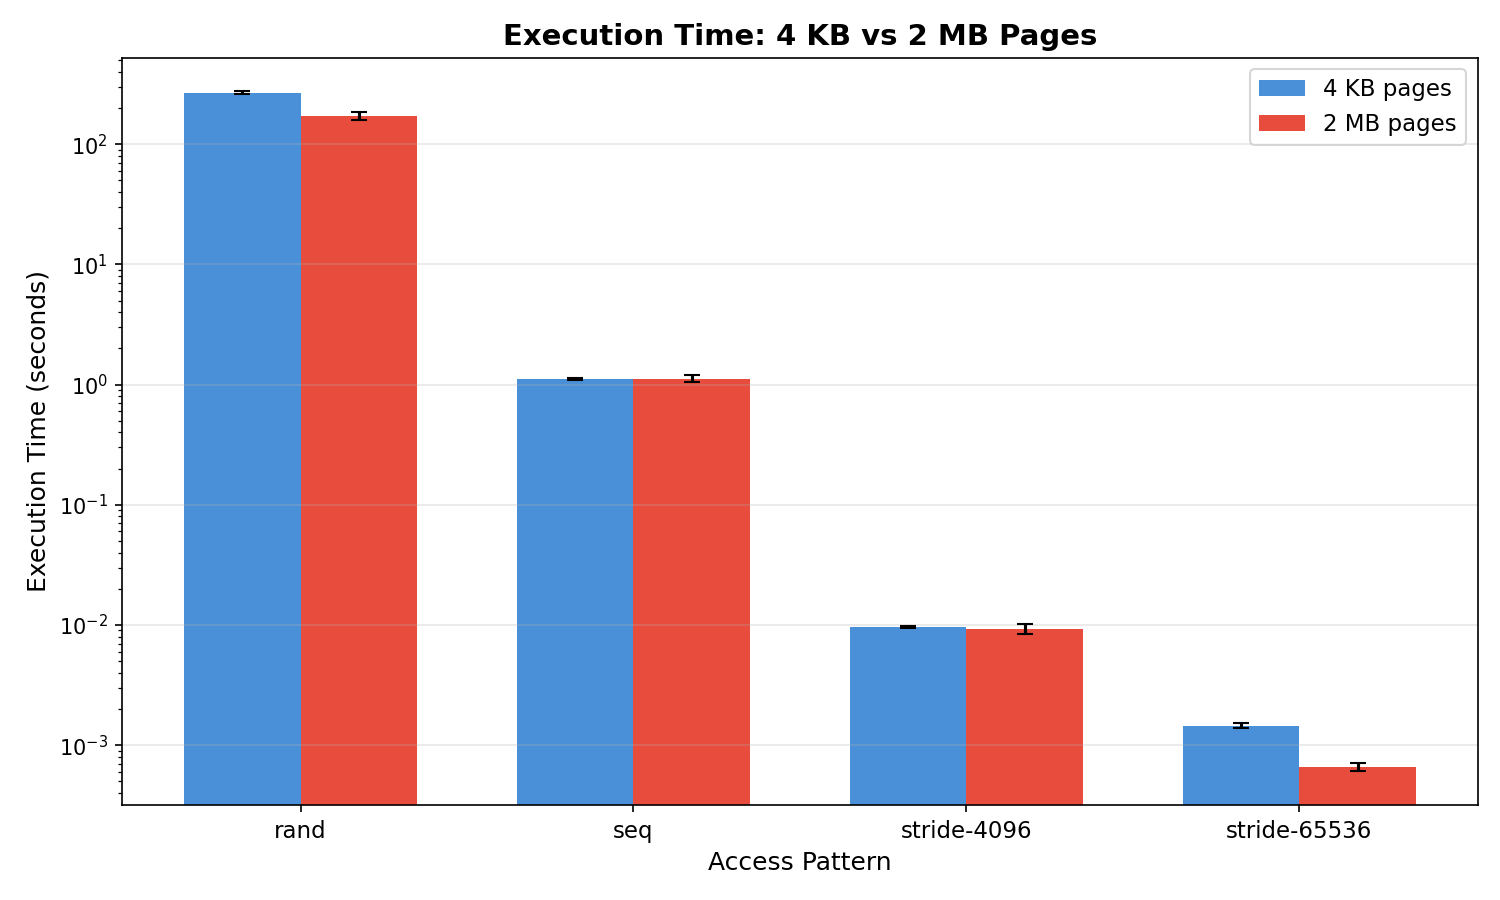
\includegraphics[width=\columnwidth]{synthetic/execution_time.png}
    \caption{Execution time comparison (synthetic workload).}
    \label{fig:syn_time}
\end{figure}

\subsubsection{Instructions Per Cycle (IPC)}
Random access IPC improved from 0.21 to 0.32 (+52.4\%) with huge pages, showing that TLB misses were a major pipeline bottleneck. Sequential access achieved high IPC ($>$3.5) in both configurations, confirming spatial locality.

\begin{figure}[H]
    \centering
    
\includegraphics[width=\columnwidth]{synthetic/ipc.png}
    \caption{IPC comparison across access patterns (synthetic workload).}
    \label{fig:syn_ipc}
\end{figure}

\begin{figure}[H]
    \centering
    
\includegraphics[width=\columnwidth]{synthetic/cpu_cycles.png}
    \caption{CPU cycles comparison (synthetic workload).}
    \label{fig:syn_cycles}
\end{figure}

\begin{figure}[H]
    \centering
    
\includegraphics[width=\columnwidth]{synthetic/improvement_summary.png}
    \caption{Percentage improvement summary with 2\,MB pages (synthetic workload).}
    \label{fig:syn_improvement}
\end{figure}

\subsection{Analysis}

\textbf{Why random access benefits most:} Each random access potentially touches a different 4\,KB page. With $\sim$1,500 TLB entries and 262,144 pages in the working set, the TLB hit rate is effectively zero. Huge pages reduce the address space to $\sim$512 pages, making it far more TLB-friendly.

\textbf{Why sequential access shows no improvement:} Sequential access fully utilizes each page before moving to the next. A single TLB miss covers 4,096 (4\,KB) or 2,097,152 (2\,MB) consecutive byte accesses; in both cases, the per-access TLB miss rate is negligible.

\textbf{Page faults vs.\ TLB misses:} Page faults are a one-time cost during initial memory population. TLB misses are ongoing during execution. For long-running workloads, \emph{TLB miss reduction} is the dominant performance driver, not page fault reduction.

% ============================================================
% V. WEB SERVER WORKLOAD
% ============================================================
\section{Web Server Workload}

\subsection{Workload Design}

The web server experiments use \textbf{nginx 1.24.0} configured for static file serving with \texttt{sendfile on}, \texttt{tcp\_nopush on}, and logging disabled. Load is generated using \textbf{wrk 4.1.0} with 4 threads in \texttt{--latency} mode, running locally on port 8088 to eliminate network variability.

\textbf{Test data:} 500 small files ($\sim$6.9\,KB HTML each) and 10 large files (50\,MB binary each). Page configurations are 4\,KB (THP=\texttt{never}) vs.\ 2\,MB (THP=\texttt{always}). Each run lasts 30 seconds with 3 repetitions, for a total of \textbf{48 runs} (2 file sizes $\times$ 2 concurrency levels $\times$ 2 page configs $\times$ 2 cache states $\times$ 3 repetitions).

\subsection{Results}

\subsubsection{Small File Serving ($\sim$7\,KB)}

\begin{table}[H]
\centering
\caption{Small File Serving Results}
\label{tab:web_small}
\resizebox{\columnwidth}{!}{%
\begin{tabular}{@{}lrrrrrr@{}}
\toprule
\textbf{Config} & \textbf{Req/s} & \textbf{Avg Lat ($\mu$s)} & \textbf{p99 ($\mu$s)} & \textbf{PF} & \textbf{dTLB-L} & \textbf{IPC} \\
\midrule
c10-4KB-cold  & 115,192 & 77    & 519   & 72  & 17.0M & 0.52 \\
c10-2MB-cold  & 63,211  & 157   & 1,360 & 77  & 21.7M & 0.44 \\
c10-4KB-warm  & 107,245 & 81    & 504   & 0   & 17.4M & 0.52 \\
c10-2MB-warm  & 67,998  & 143   & 1,230 & 0   & 21.0M & 0.45 \\
c200-4KB-cold & 150,130 & 1,353 & 6,383 & 156 & 56.3M & 0.49 \\
c200-2MB-cold & 92,162  & 2,110 & 9,433 & 153 & 44.6M & 0.42 \\
c200-4KB-warm & 145,620 & 1,353 & 6,233 & 2   & 57.5M & 0.49 \\
c200-2MB-warm & 79,493  & 2,390 & 10,203& 3   & 41.4M & 0.41 \\
\bottomrule
\end{tabular}%
}
\end{table}

\subsubsection{Large File Serving (50\,MB)}

\begin{table}[H]
\centering
\caption{Large File Serving Results}
\label{tab:web_large}
\resizebox{\columnwidth}{!}{%
\begin{tabular}{@{}lrrrrrr@{}}
\toprule
\textbf{Config} & \textbf{Req/s} & \textbf{Avg Lat (ms)} & \textbf{p99 (ms)} & \textbf{PF} & \textbf{dTLB-L} & \textbf{IPC} \\
\midrule
c10-4KB-cold  & 256 & 27.2  & 77.6    & 76  & 37.1M & 0.85 \\
c10-2MB-cold  & 120 & 60.0  & 145.8   & 61  & 11.7M & 0.62 \\
c10-4KB-warm  & 273 & 32.4  & 212.9   & 1   & 41.8M & 0.87 \\
c10-2MB-warm  & 117 & 61.2  & 130.0   & 9   & 11.7M & 0.62 \\
c200-4KB-cold & 180 & 761.9 & 1,906.7 & 560 & 10.0M & 0.74 \\
c200-2MB-cold & 135 & 931.4 & 1,946.7 & 558 & 12.4M & 0.62 \\
c200-4KB-warm & 161 & 811.2 & 1,916.7 & 63  & 14.4M & 0.69 \\
c200-2MB-warm & 140 & 864.2 & 1,933.3 & 159 & 13.7M & 0.62 \\
\bottomrule
\end{tabular}%
}
\end{table}

\subsection{Key Findings}

\subsubsection{4\,KB Pages Consistently Outperform 2\,MB Pages}
This is the most striking result. Unlike the synthetic workload, 4\,KB pages delivered \textbf{42--133\% higher throughput} than 2\,MB pages across all configurations (Table~\ref{tab:web_advantage}).

\begin{table}[H]
\centering
\caption{Throughput Advantage of 4\,KB Pages (Web Server)}
\label{tab:web_advantage}
\begin{tabular}{@{}lrrr@{}}
\toprule
\textbf{Config} & \textbf{4KB} & \textbf{2MB} & \textbf{4KB Adv.} \\
\midrule
Small, c10, cold  & 115,192 & 63,211 & +82\%  \\
Small, c10, warm  & 107,245 & 67,998 & +58\%  \\
Small, c200, cold & 150,130 & 92,162 & +63\%  \\
Small, c200, warm & 145,620 & 79,493 & +83\%  \\
Large, c10, cold  & 256     & 120    & +113\% \\
Large, c10, warm  & 273     & 117    & +133\% \\
Large, c200, cold & 180     & 135    & +33\%  \\
Large, c200, warm & 161     & 140    & +15\%  \\
\bottomrule
\end{tabular}
\end{table}

\begin{figure}[H]
    \centering
    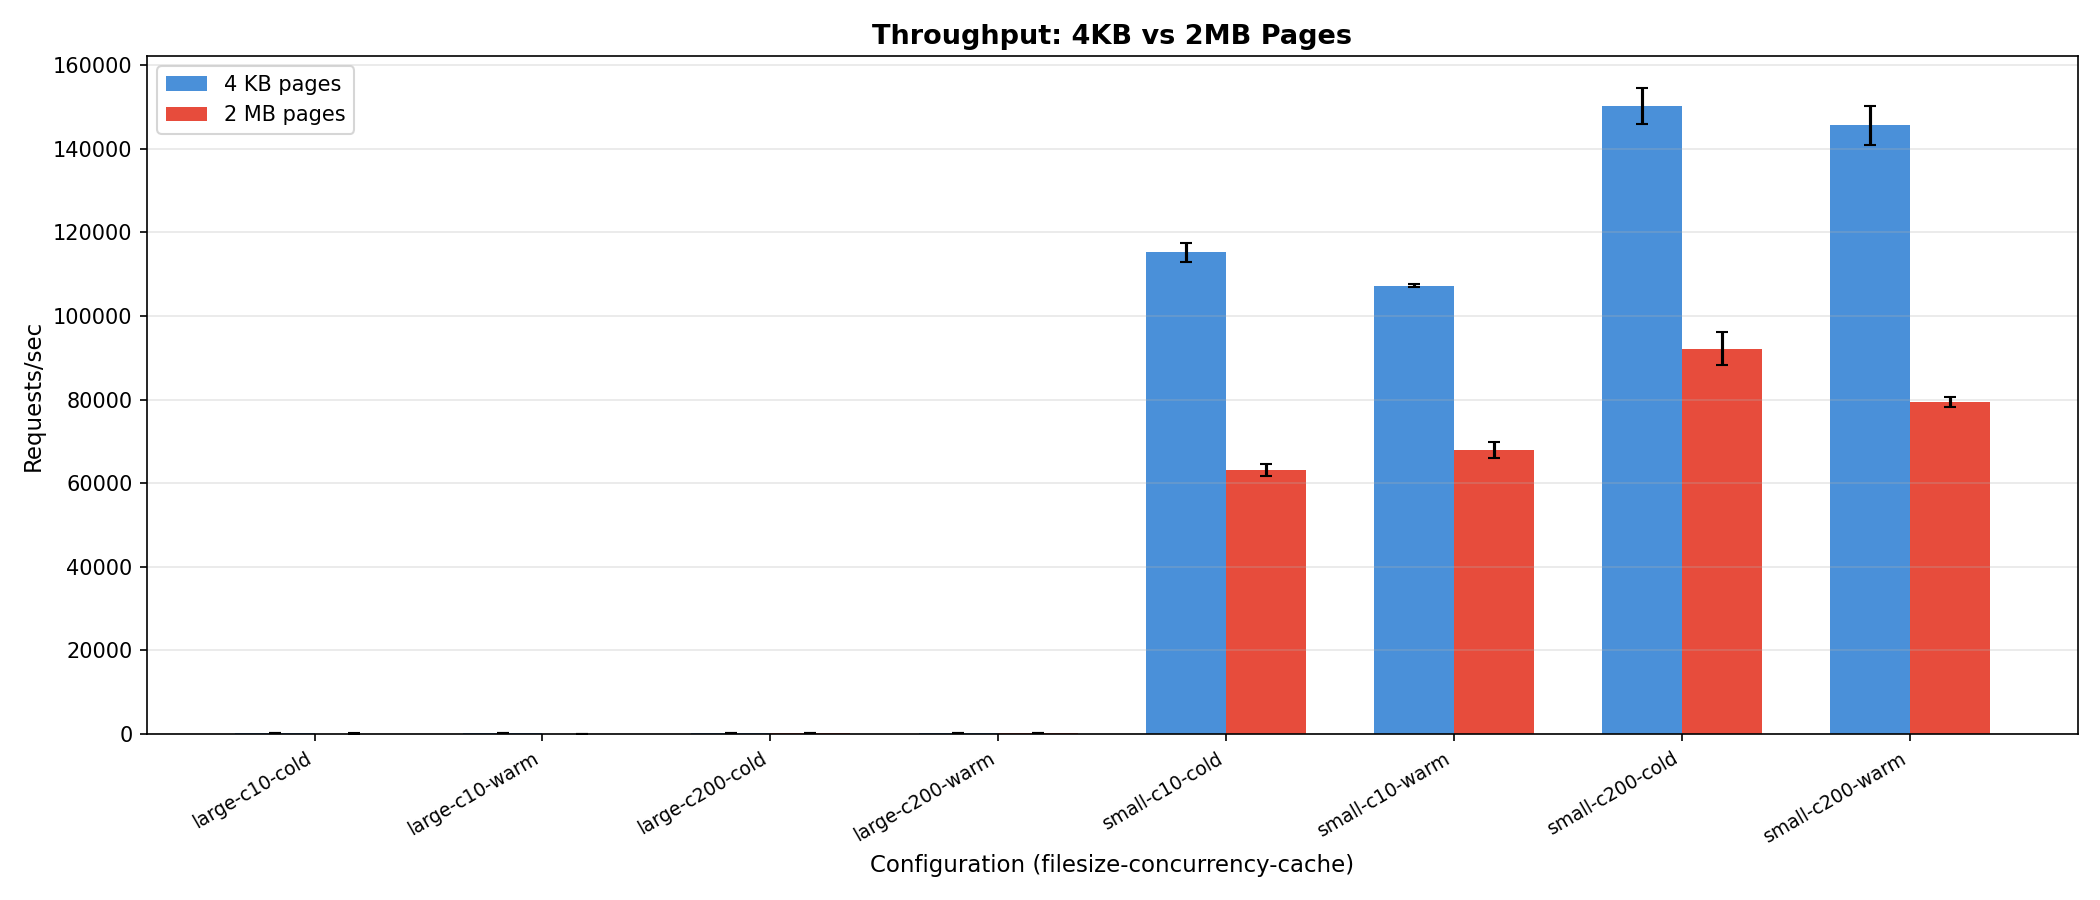
\includegraphics[width=\columnwidth]{webserver/throughput.png}
    \caption{Request throughput: 4\,KB vs 2\,MB pages (web server).}
    \label{fig:web_throughput}
\end{figure}

\begin{figure}[H]
    \centering
    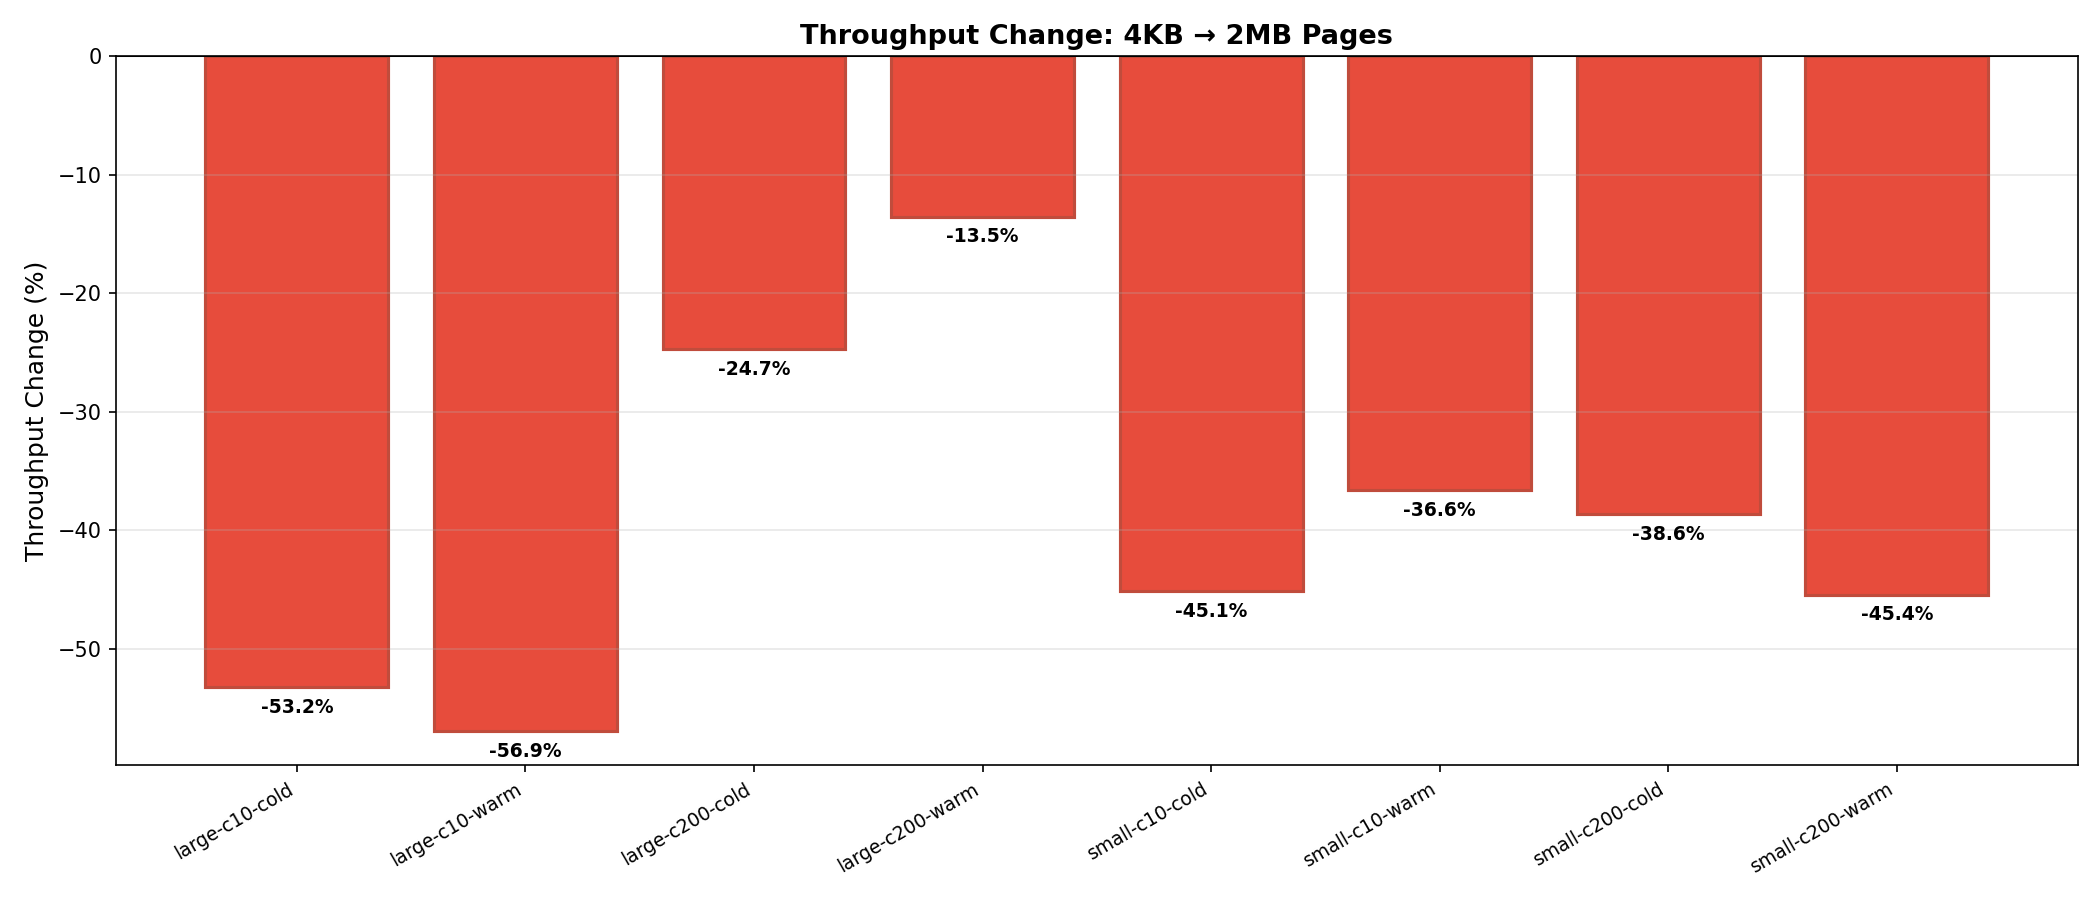
\includegraphics[width=\columnwidth]{webserver/throughput_change.png}
    \caption{Percentage throughput change with 2\,MB pages (web server).}
    \label{fig:web_throughput_change}
\end{figure}

\subsubsection{Page Faults Are Not the Bottleneck}
Page faults were extremely low ($\sim$60--160 for cold, $\sim$0 for warm), confirming that nginx and the OS page cache handle demand paging efficiently.

\begin{figure}[H]
    \centering
    
\includegraphics[width=\columnwidth]{webserver/page_faults.png}
    \caption{Page faults comparison (web server).}
    \label{fig:web_pf}
\end{figure}

\subsubsection{Mixed TLB Behavior}
Unlike synthetic workloads, dTLB load misses did \emph{not} consistently decrease with huge pages. For small files, dTLB misses \emph{increased} (17M $\rightarrow$ 22M at c10). For large files, dTLB misses \emph{decreased} (37M $\rightarrow$ 12M) but throughput still dropped.

\begin{figure}[H]
    \centering
    
\includegraphics[width=\columnwidth]{webserver/dtlb_load_misses.png}
    \caption{dTLB load misses (web server).}
    \label{fig:web_dtlb}
\end{figure}

\subsubsection{iTLB Pollution with Huge Pages}
A critical observation: iTLB load misses were significantly elevated with 2\,MB pages for small files. Huge pages for data regions displace instruction TLB entries, causing instruction fetch stalls.

\begin{figure}[H]
    \centering
    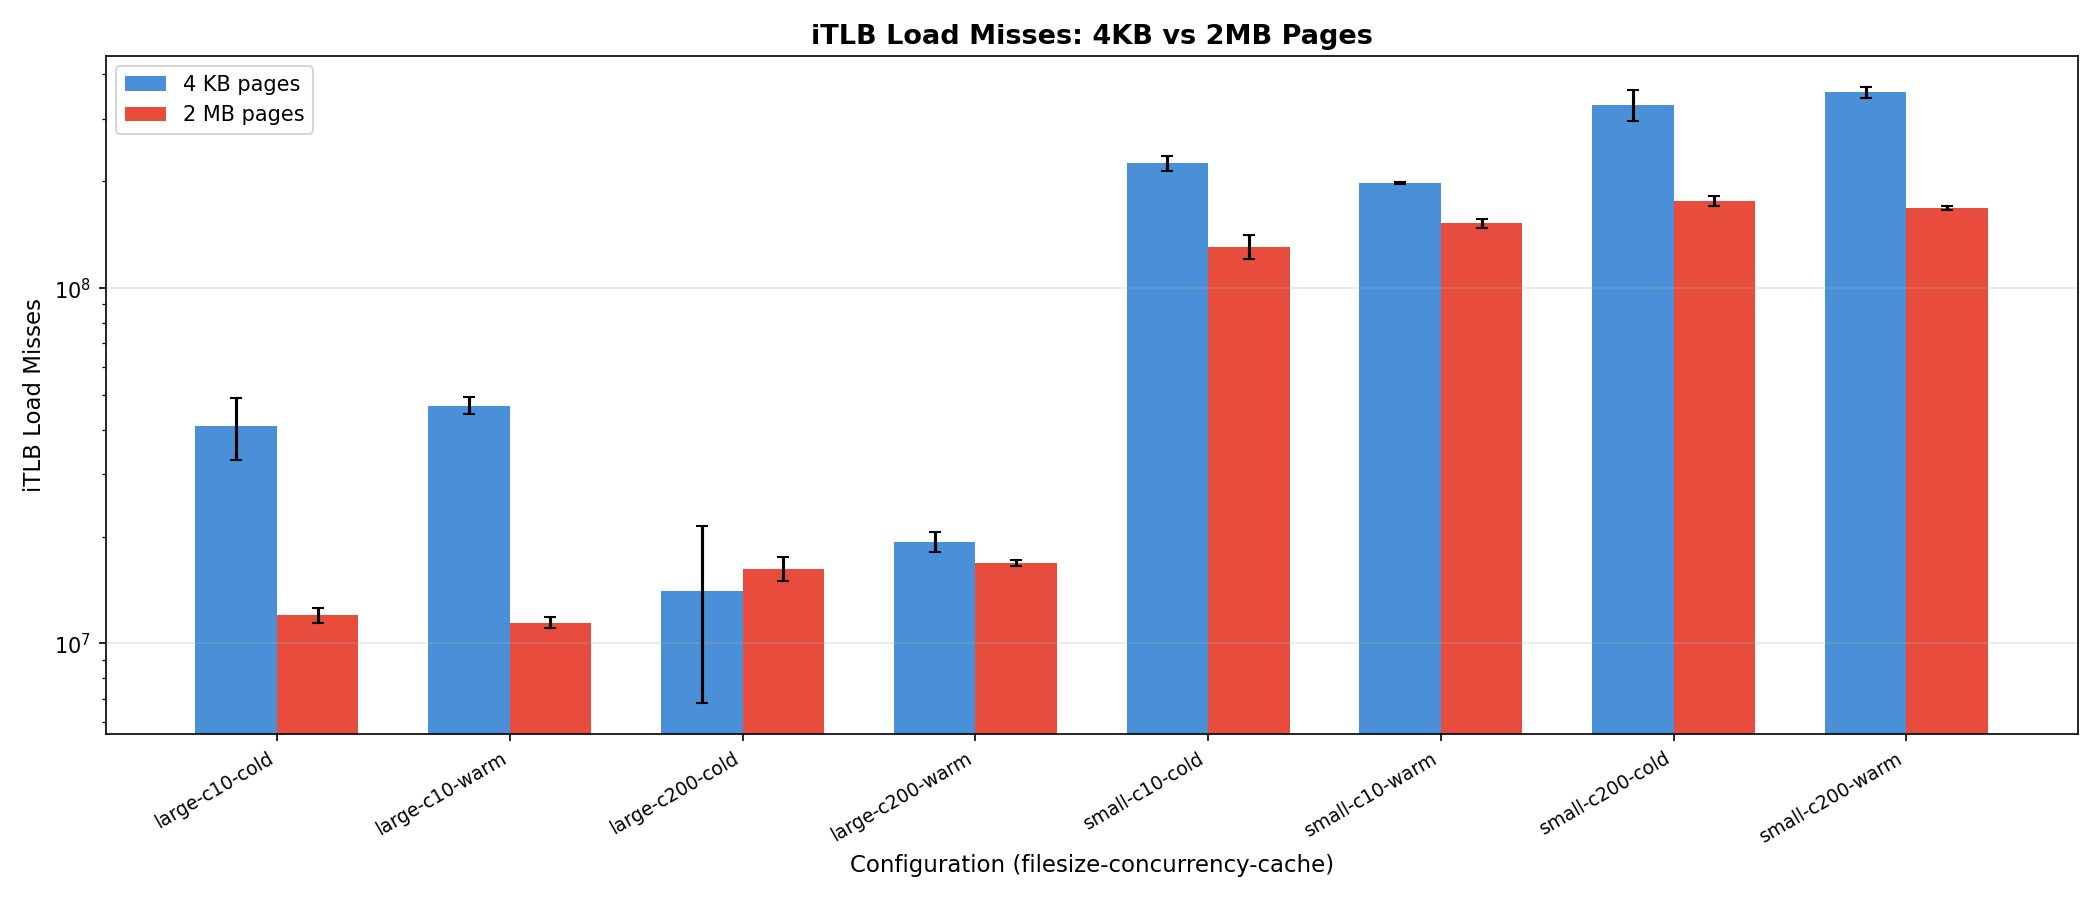
\includegraphics[width=\columnwidth]{webserver/itlb_load_misses.png}
    \caption{iTLB load misses (web server).}
    \label{fig:web_itlb}
\end{figure}

\subsubsection{IPC and Latency}
IPC was consistently lower with 2\,MB pages (--14\% to --27\%), indicating increased pipeline stalls despite fewer dTLB misses for data. Latency roughly doubled across most configurations.

\begin{figure}[H]
    \centering
    
\includegraphics[width=\columnwidth]{webserver/ipc.png}
    \caption{IPC comparison (web server).}
    \label{fig:web_ipc}
\end{figure}

\begin{figure}[H]
    \centering
    
\includegraphics[width=\columnwidth]{webserver/latency_avg.png}
    \caption{Average latency comparison (web server).}
    \label{fig:web_lat_avg}
\end{figure}

\begin{figure}[H]
    \centering
    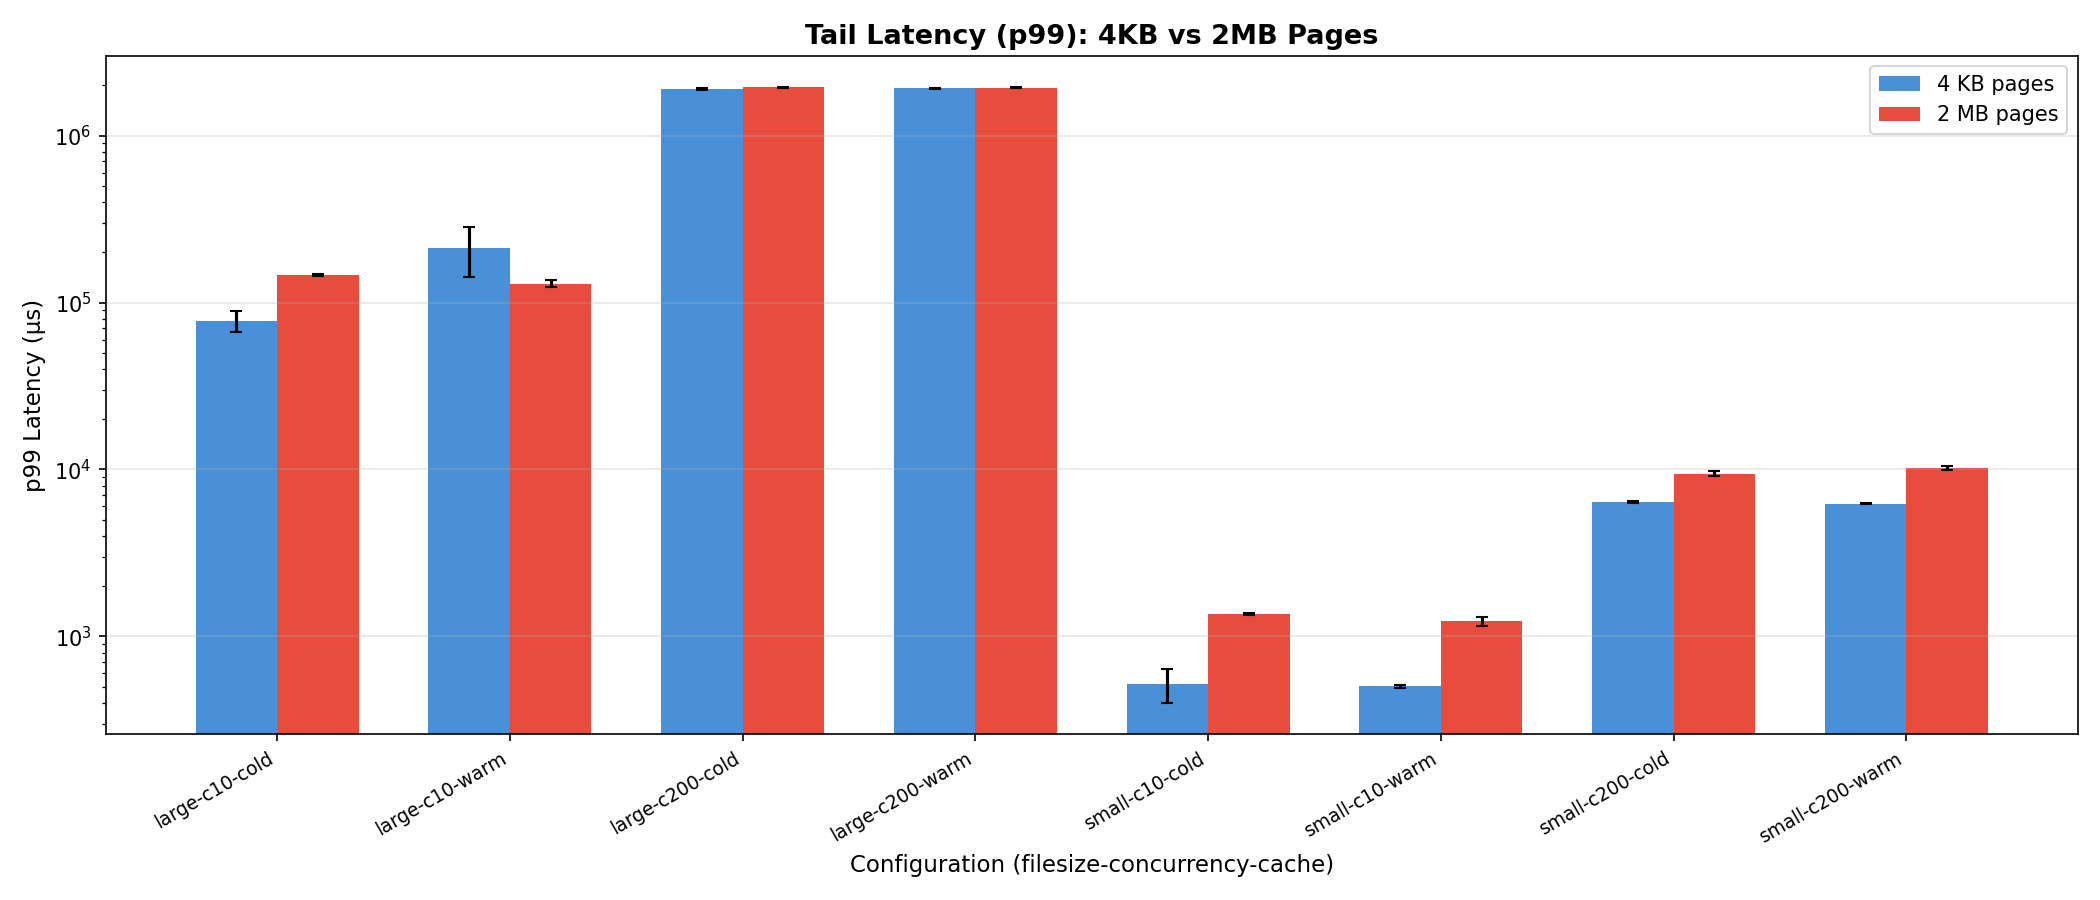
\includegraphics[width=\columnwidth]{webserver/latency_p99.png}
    \caption{p99 tail latency comparison (web server).}
    \label{fig:web_lat_p99}
\end{figure}

\begin{figure}[H]
    \centering
    
\includegraphics[width=\columnwidth]{webserver/cpu_cycles.png}
    \caption{CPU cycles comparison (web server).}
    \label{fig:web_cycles}
\end{figure}

\subsection{Analysis}

Several factors explain why 4\,KB pages outperform 2\,MB pages for nginx:

\begin{enumerate}
    \item \textbf{Memory access pattern}: nginx serves files via \texttt{sendfile()}, performing sequential reads through the page cache. Data is copied from page cache to socket buffers via DMA---minimal TLB-dependent user-space memory access occurs.
    \item \textbf{Internal fragmentation}: small files ($\sim$7\,KB) occupy 2 pages at 4\,KB but waste most of a 2\,MB huge page, reducing effective memory utilization and cache efficiency.
    \item \textbf{THP overhead}: with THP set to \texttt{always}, the kernel's \texttt{khugepaged} daemon actively compacts and promotes pages, consuming CPU cycles and causing latency spikes.
    \item \textbf{iTLB pollution}: huge pages for data regions displace instruction TLB entries. nginx's HTTP handling involves complex branching that is sensitive to iTLB misses.
    \item \textbf{Page table walk cost}: for nginx's working set (many small files + connection state), the 4\,KB page table structure is more cache-friendly.
\end{enumerate}

% ============================================================
% VI. DATABASE WORKLOAD
% ============================================================
\section{Database Workload}

\subsection{Workload Design}

The database experiments use \textbf{PostgreSQL 16} with \textbf{sysbench 1.0.20} OLTP benchmarks. The dataset consists of 4 tables $\times$ 1,000,000 rows ($\sim$1.5\,GB). Each run lasts 60 seconds with 4 threads and 3 repetitions, for a total of \textbf{36 runs} (3 workloads $\times$ 2 page configs $\times$ 2 cache states $\times$ 3 repetitions).

\textbf{Workloads tested:}
\begin{itemize}
    \item \textbf{Read-only (OLTP)}: 14 SELECT queries per transaction (point lookups + range queries).
    \item \textbf{Read-write (OLTP)}: SELECT, UPDATE, INSERT, DELETE (20 queries per transaction).
    \item \textbf{Range scan}: range queries over contiguous key ranges (100-row ranges).
\end{itemize}

\subsection{Results}

\begin{table}[H]
\centering
\caption{Database Workload Results Summary}
\label{tab:db_results}
\resizebox{\columnwidth}{!}{%
\begin{tabular}{@{}lrrrrrr@{}}
\toprule
\textbf{Config} & \textbf{TPS} & \textbf{QPS} & \textbf{Avg (ms)} & \textbf{p95 (ms)} & \textbf{PF} & \textbf{IPC} \\
\midrule
RO-4KB-cold  & 1,745 & 27,913 & 2.29 & 3.31 & 1,060 & 0.89 \\
RO-2MB-cold  & 1,376 & 22,023 & 2.90 & 4.20 & 1,058 & 0.90 \\
RO-4KB-warm  & 1,891 & 30,259 & 2.11 & 2.84 & 13    & 1.16 \\
RO-2MB-warm  & 1,331 & 21,291 & 3.01 & 4.34 & 12    & 0.92 \\
\midrule
RW-4KB-cold  & 1,175 & 23,504 & 3.40 & 4.41 & 3,262 & 0.58 \\
RW-2MB-cold  & 930   & 18,601 & 4.30 & 5.95 & 3,317 & 0.48 \\
RW-4KB-warm  & 1,000 & 20,005 & 4.00 & 5.51 & 715   & 0.47 \\
RW-2MB-warm  & 916   & 18,326 & 4.37 & 6.15 & 723   & 0.47 \\
\midrule
Range-4KB-cold & 7,434 & 22,301 & 0.54 & 0.95 & 1,965 & 0.73 \\
Range-2MB-cold & 6,743 & 20,230 & 0.59 & 1.05 & 2,030 & 0.69 \\
Range-4KB-warm & 7,531 & 22,592 & 0.53 & 0.93 & 13    & 0.90 \\
Range-2MB-warm & 7,502 & 22,505 & 0.53 & 0.93 & 224   & 0.81 \\
\bottomrule
\end{tabular}%
}
\end{table}

\subsection{Key Findings}

\subsubsection{4\,KB Pages Outperform 2\,MB Pages}

4\,KB pages provide 9--42\% higher throughput for point lookup workloads, with the gap widening in warm-cache scenarios. Range scans show negligible difference.

\begin{table}[H]
\centering
\caption{TPS Advantage of 4\,KB Pages (Database)}
\label{tab:db_advantage}
\begin{tabular}{@{}lrrr@{}}
\toprule
\textbf{Workload} & \textbf{4KB} & \textbf{2MB} & \textbf{4KB Adv.} \\
\midrule
Read-only, cold  & 1,745 & 1,376 & +27\% \\
Read-only, warm  & 1,891 & 1,331 & +42\% \\
Read-write, cold & 1,175 & 930   & +26\% \\
Read-write, warm & 1,000 & 916   & +9\%  \\
Range, cold      & 7,434 & 6,743 & +10\% \\dTLB misses by 77--98\%
Range, warm      & 7,531 & 7,502 & +0.4\%\\
\bottomrule
\end{tabular}
\end{table}

\begin{figure}[H]
    \centering
    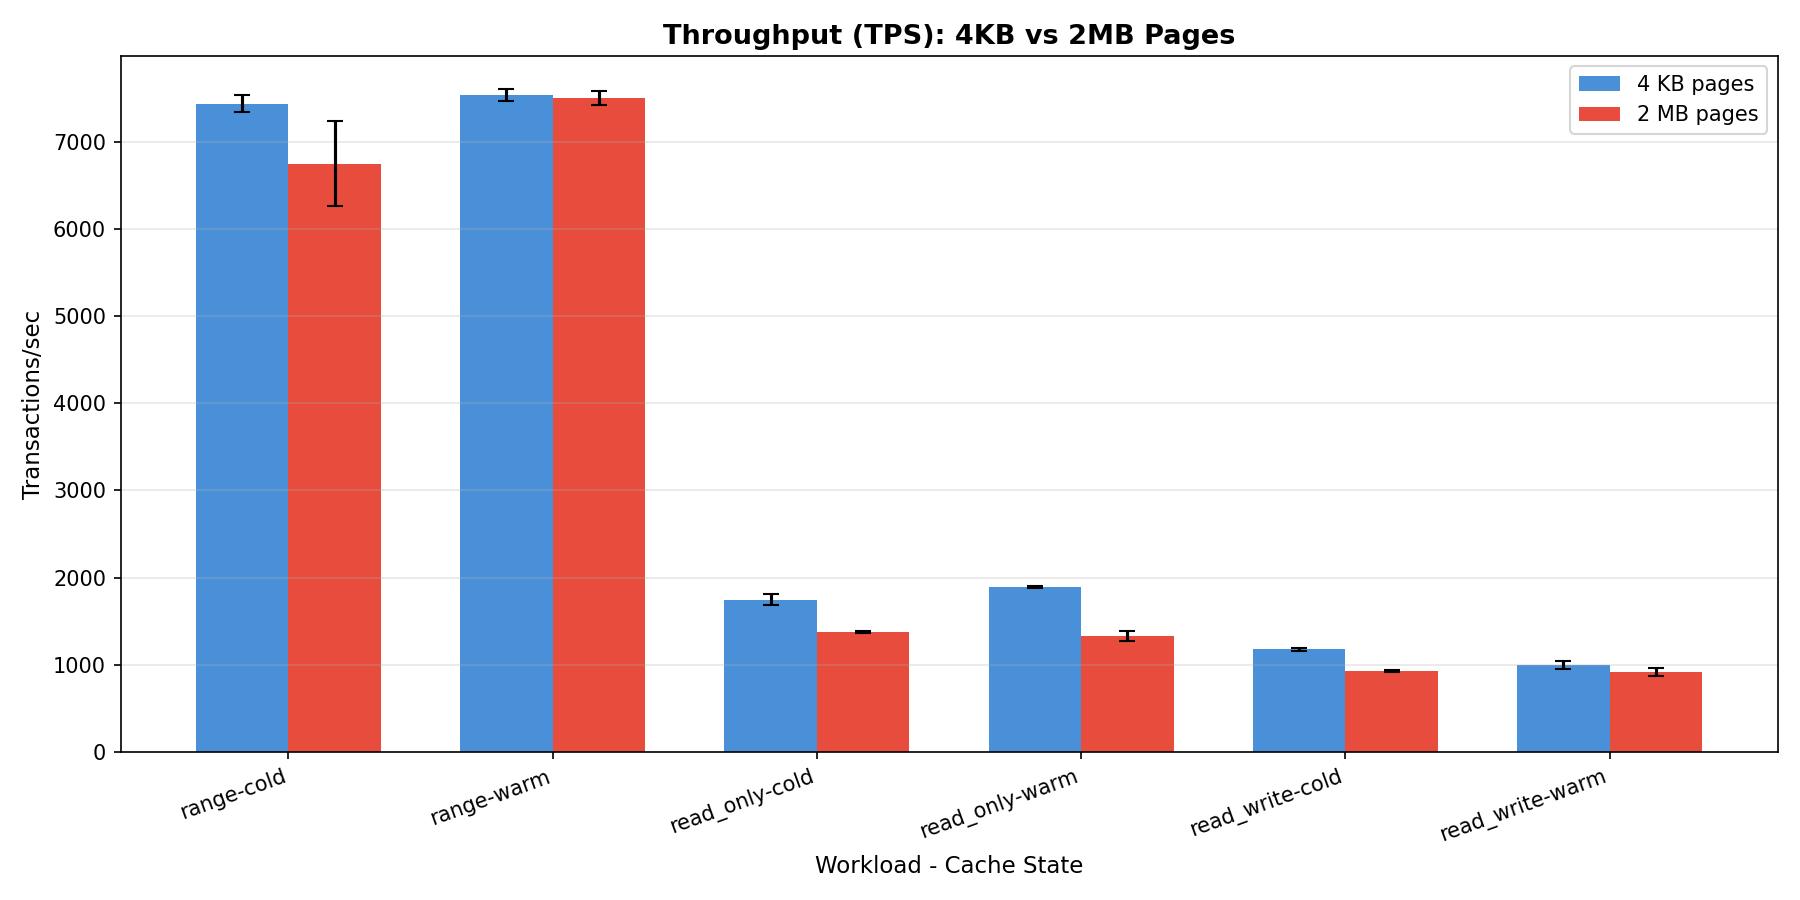
\includegraphics[width=\columnwidth]{database/tps.png}
    \caption{Transactions per second: 4\,KB vs 2\,MB pages (database).}
    \label{fig:db_tps}
\end{figure}

\begin{figure}[H]
    \centering
    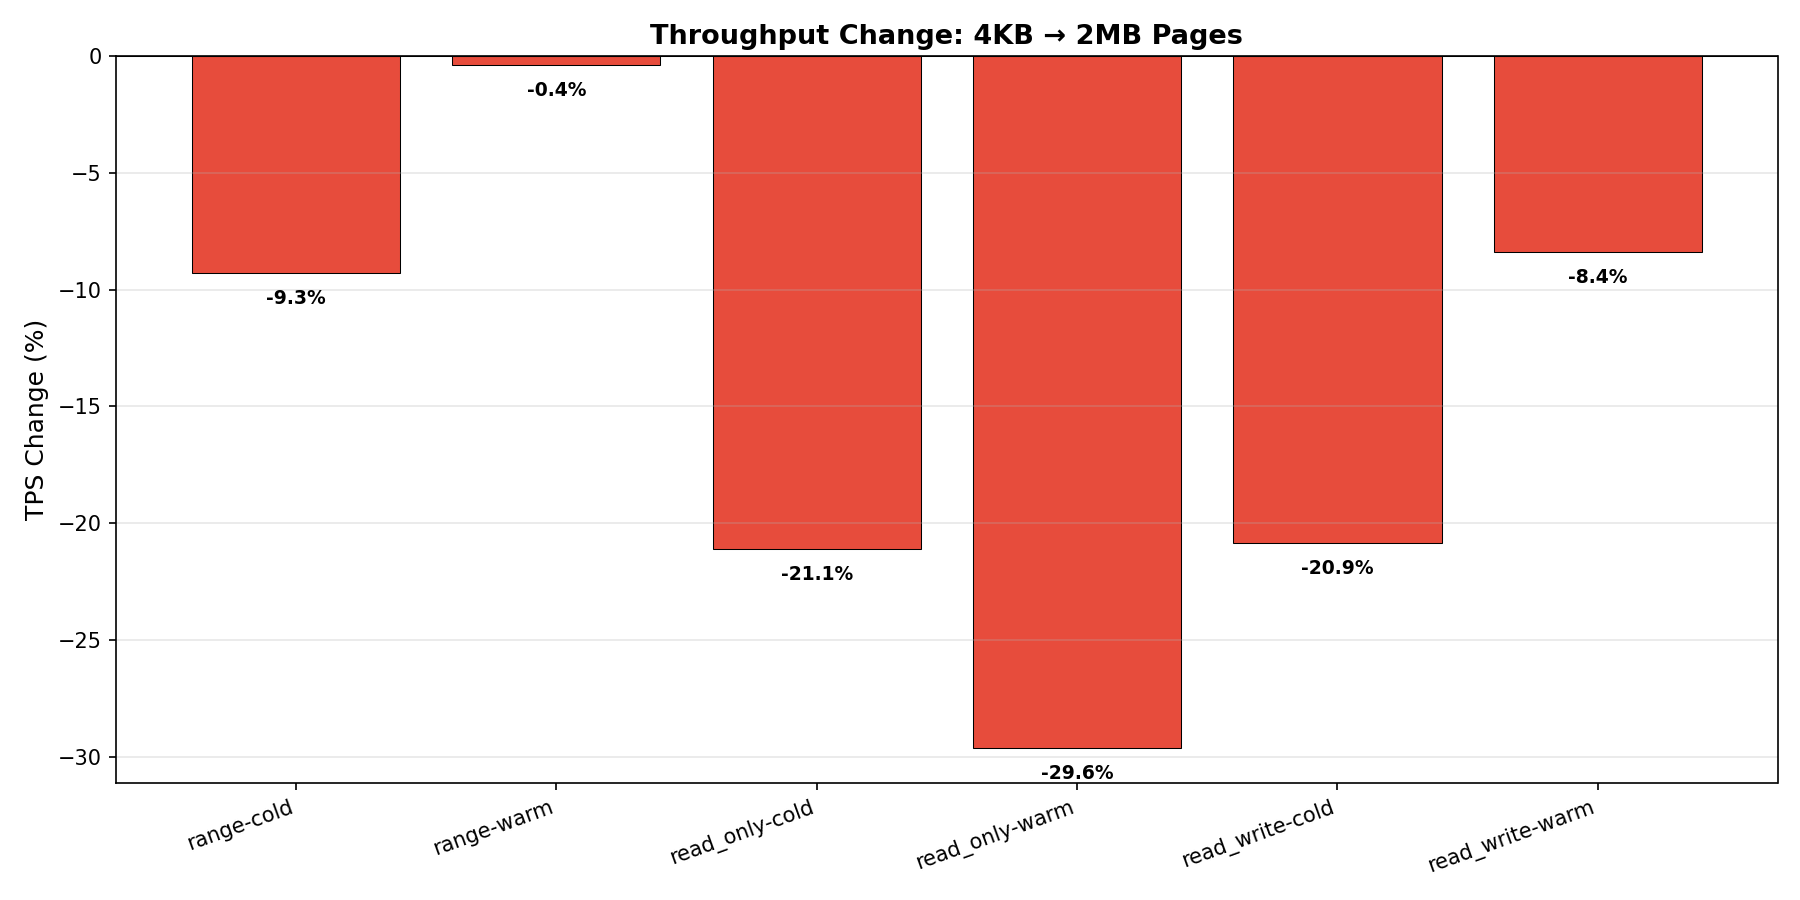
\includegraphics[width=\columnwidth]{database/tps_change.png}
    \caption{TPS percentage change with 2\,MB pages (database).}
    \label{fig:db_tps_change}
\end{figure}

\subsubsection{Page Faults Are Similar Between Configurations}
Page faults are low ($\sim$1K--3K cold, $\sim$10--700 warm) and nearly identical between configurations. PostgreSQL's internal buffer pool mediates memory access, neutralizing page fault differences.

\begin{figure}[H]
    \centering
    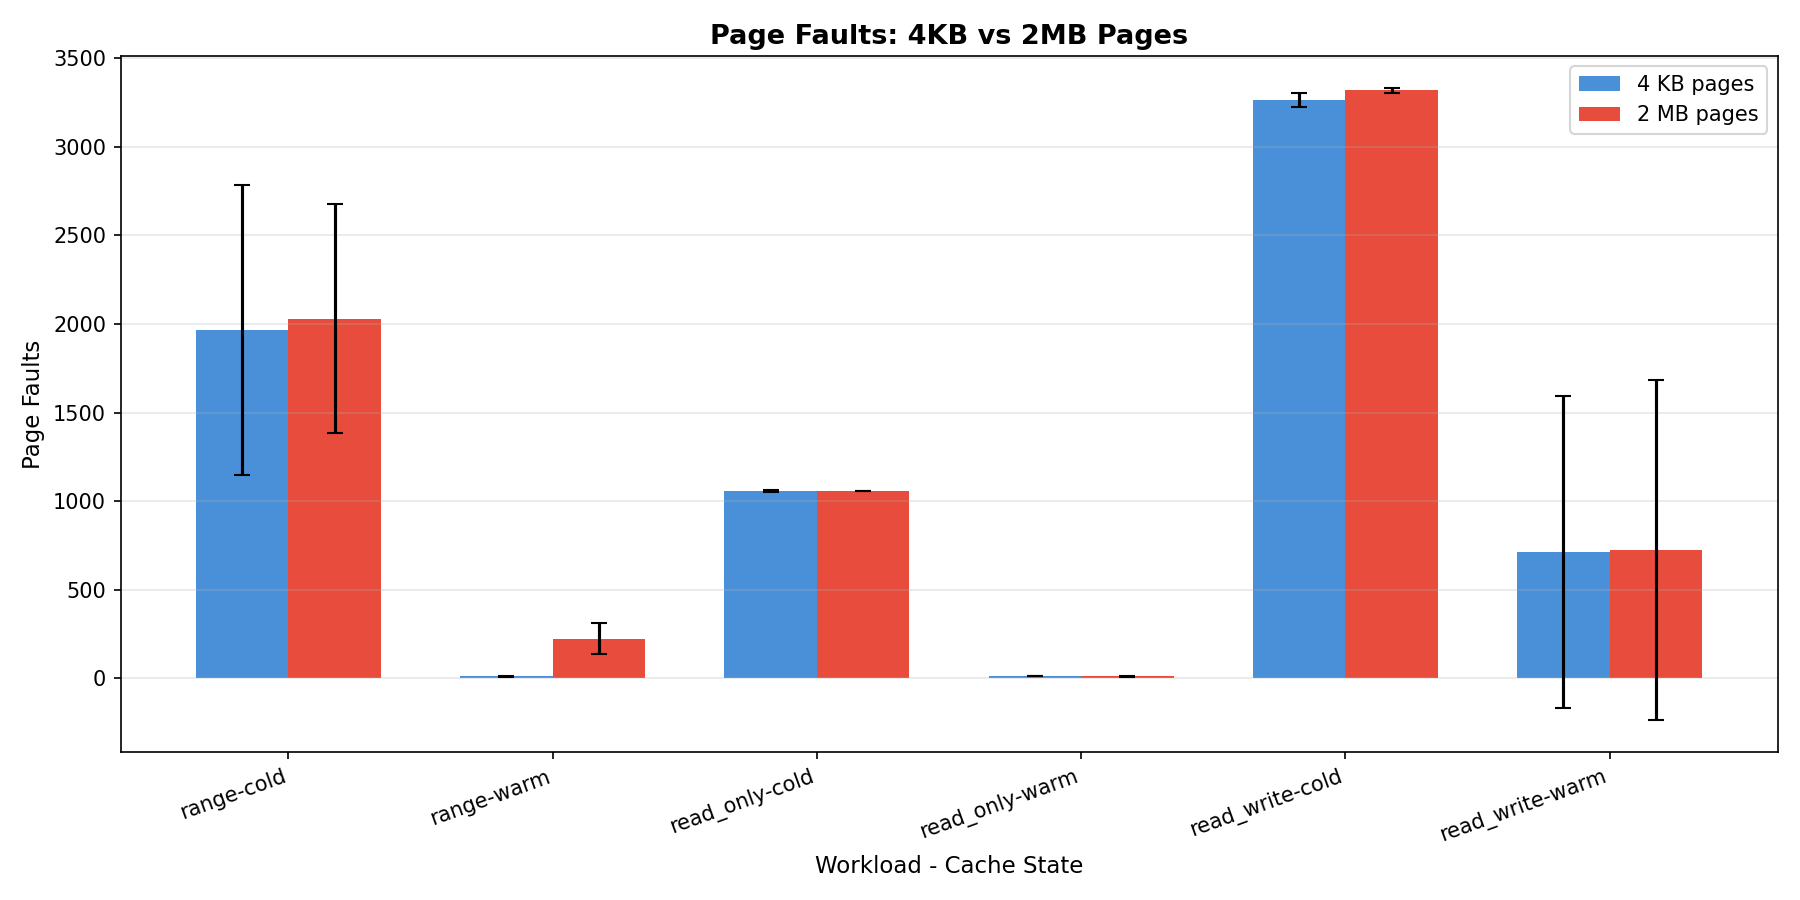
\includegraphics[width=\columnwidth]{database/page_faults.png}
    \caption{Page faults comparison (database).}
    \label{fig:db_pf}
\end{figure}

\subsubsection{Latency}
The p95 tail latency increase with 2\,MB pages is notable for read-only workloads (+27\% cold, +53\% warm), indicating THP background compaction causes latency spikes.

\begin{figure}[H]
    \centering
    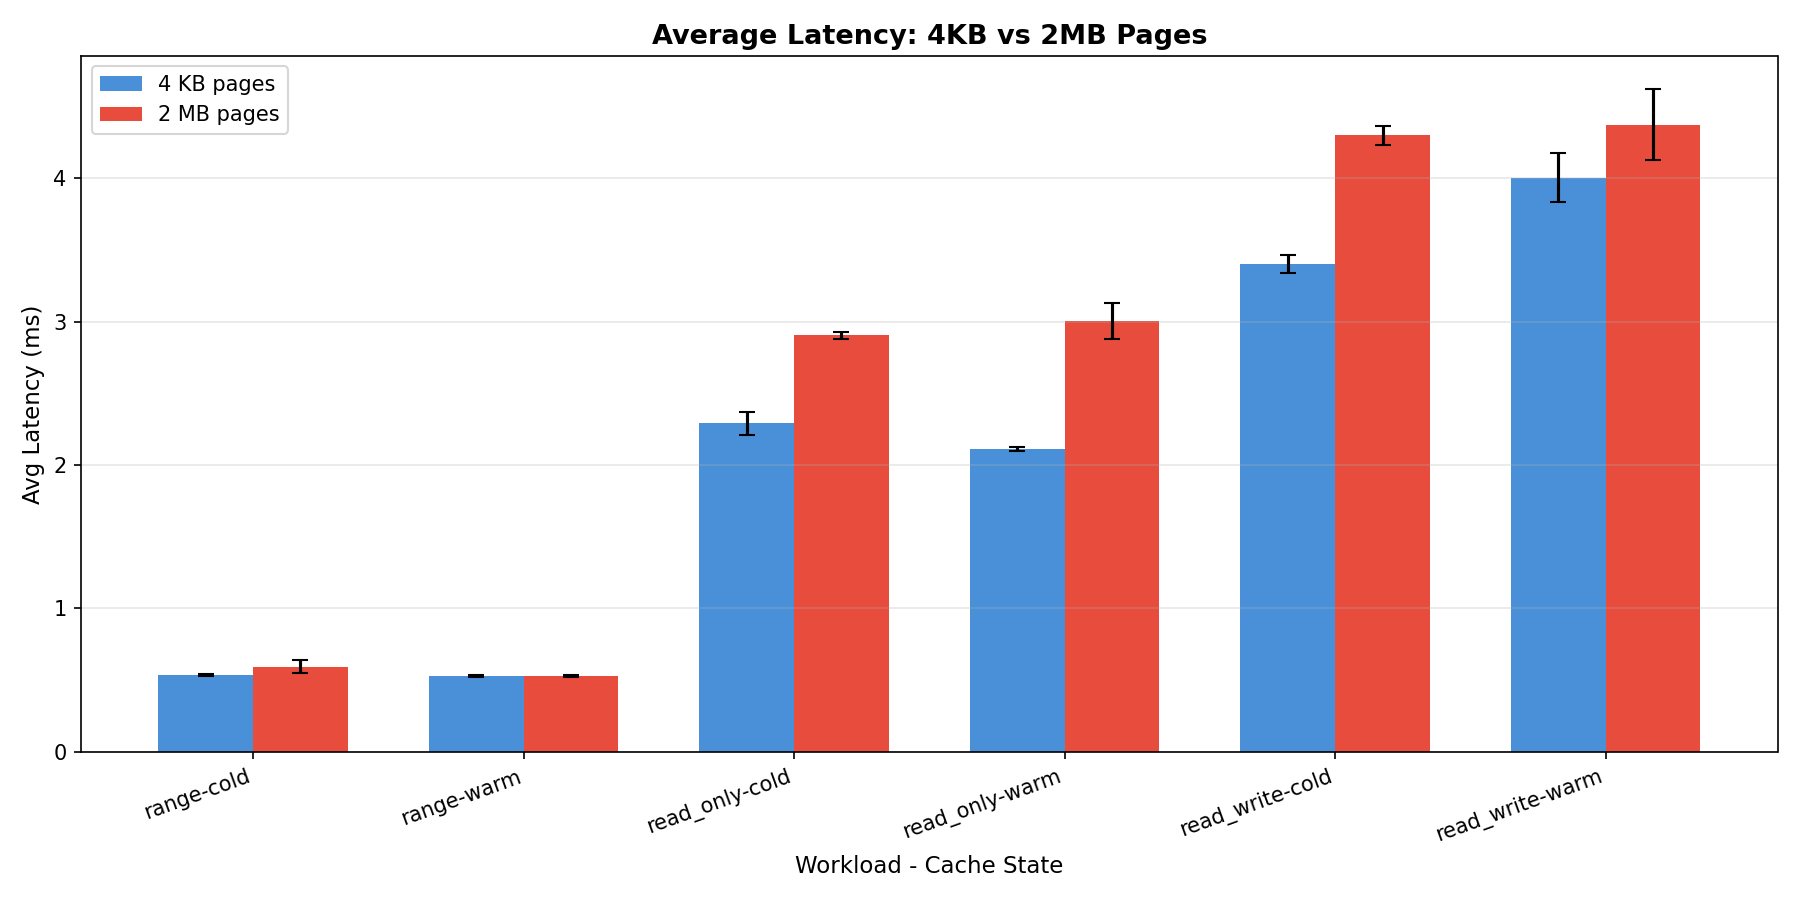
\includegraphics[width=\columnwidth]{database/latency_avg.png}
    \caption{Average latency comparison (database).}
    \label{fig:db_lat_avg}
\end{figure}

\begin{figure}[H]
    \centering
    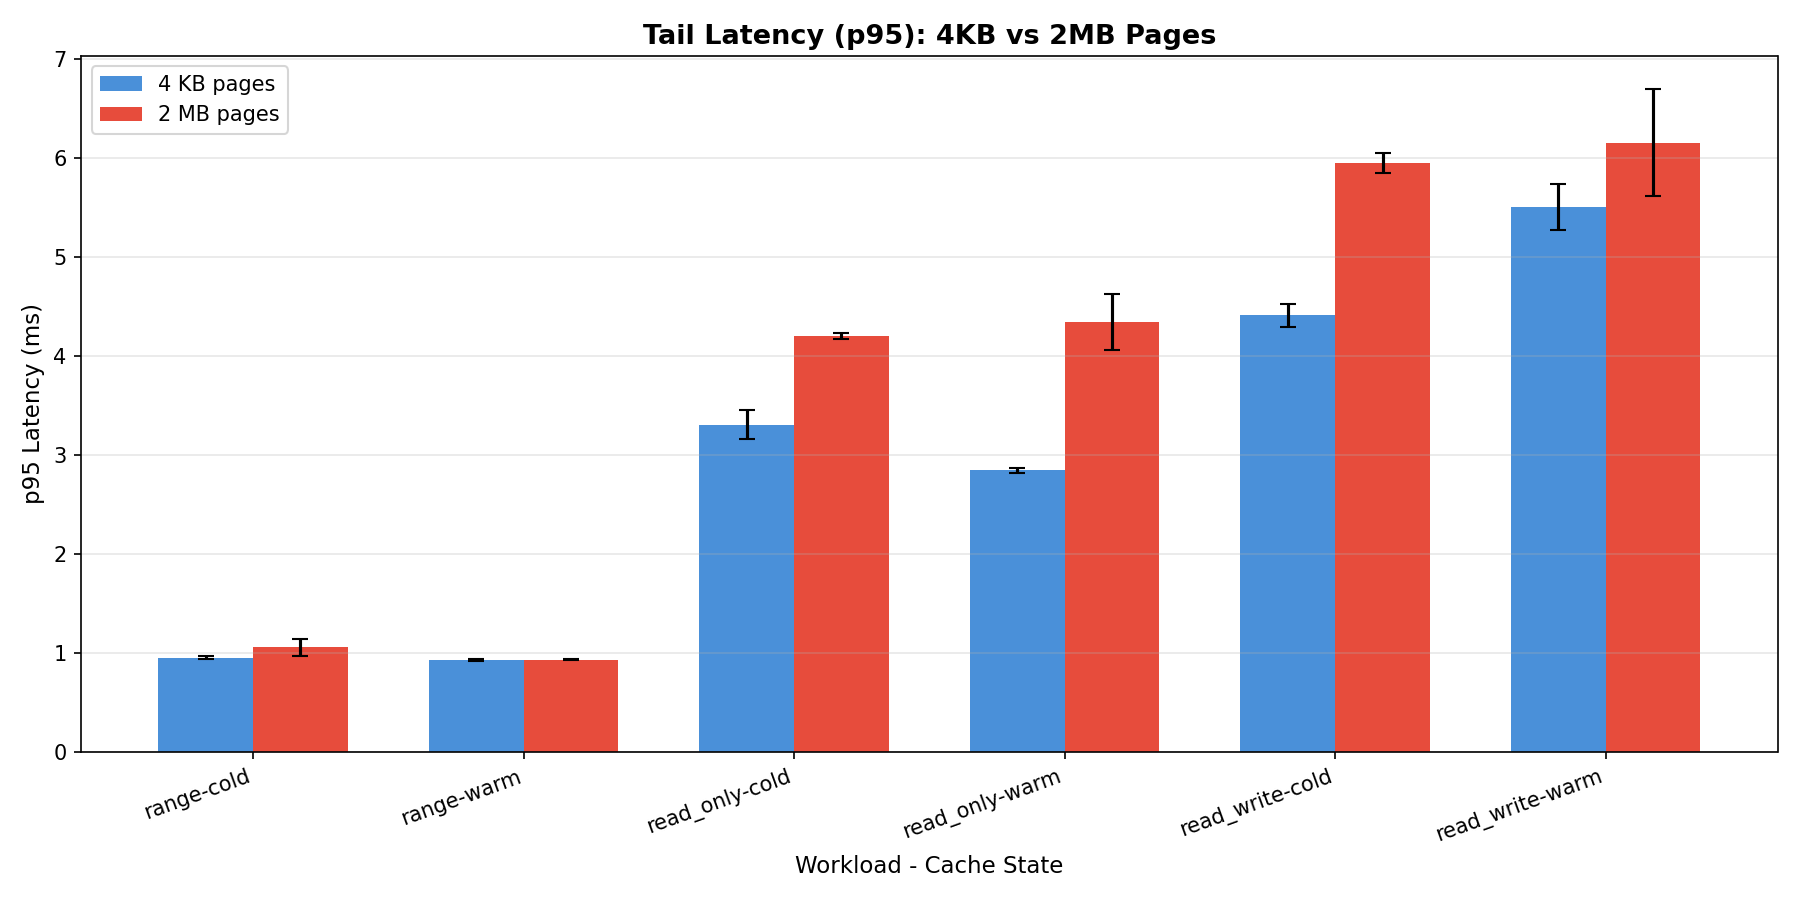
\includegraphics[width=\columnwidth]{database/latency_p95.png}
    \caption{p95 tail latency comparison (database).}
    \label{fig:db_lat_p95}
\end{figure}

\subsubsection{IPC and TLB Metrics}
In the warm read-only scenario, 4\,KB pages achieve markedly higher IPC (1.16 vs.\ 0.92), suggesting huge pages increase pipeline stalls during point lookups.

\begin{figure}[H]
    \centering
    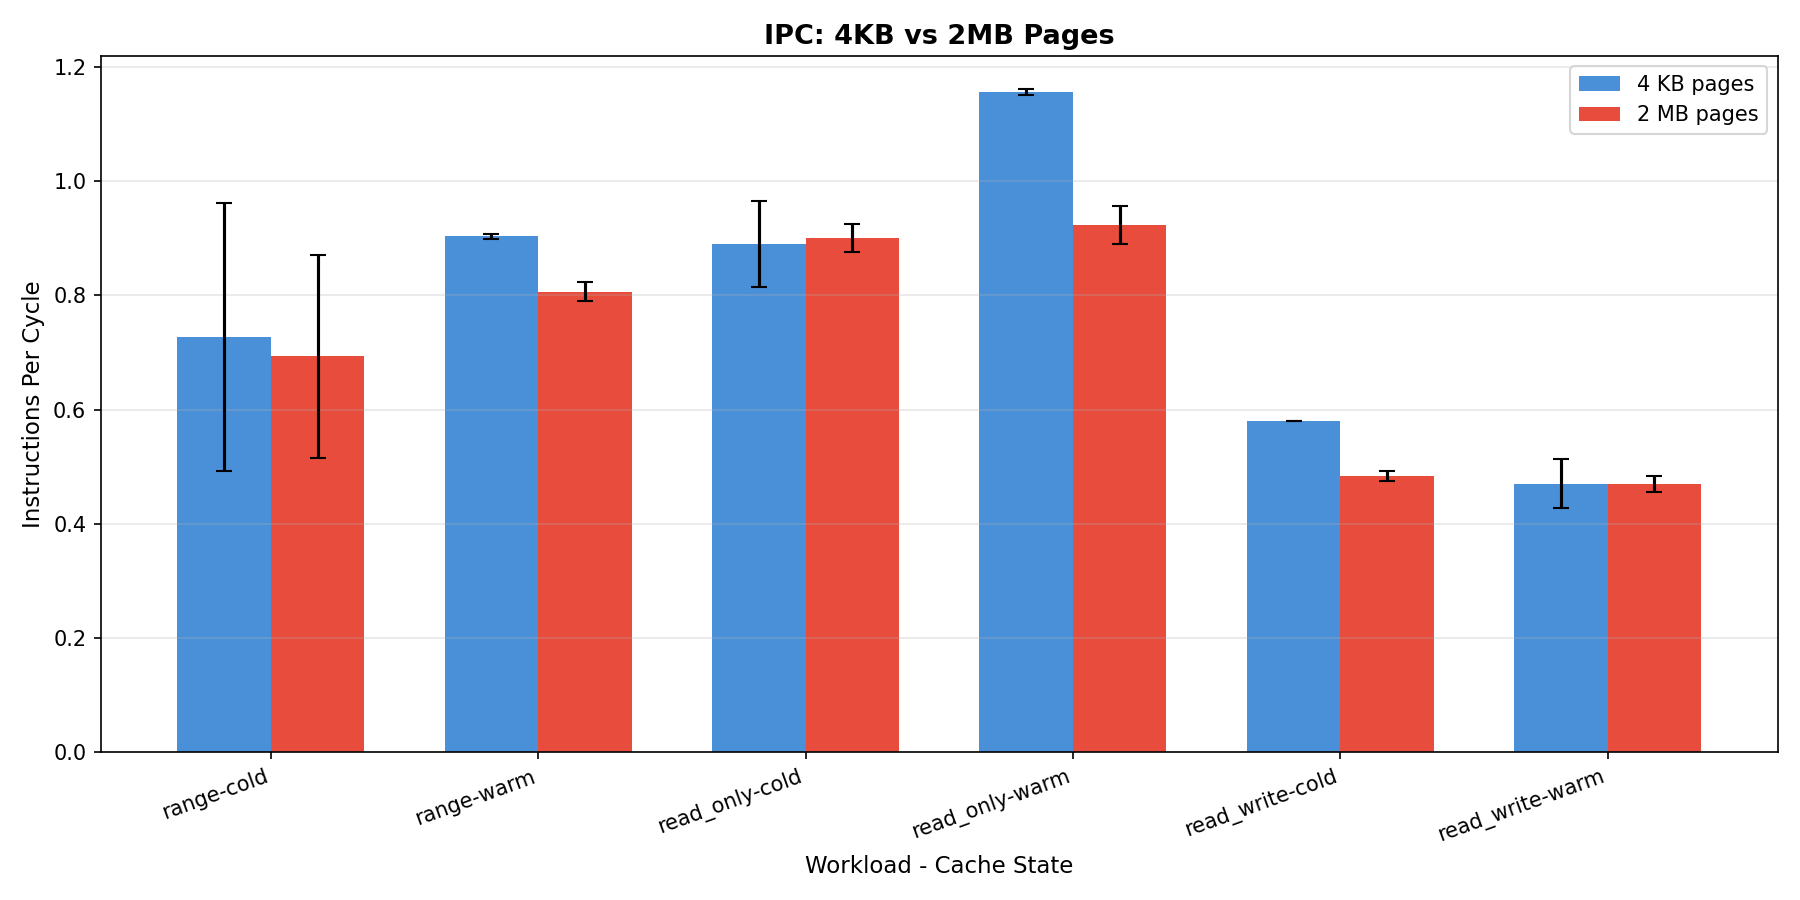
\includegraphics[width=\columnwidth]{database/ipc.png}
    \caption{IPC comparison (database).}
    \label{fig:db_ipc}
\end{figure}

\begin{figure}[H]
    \centering
    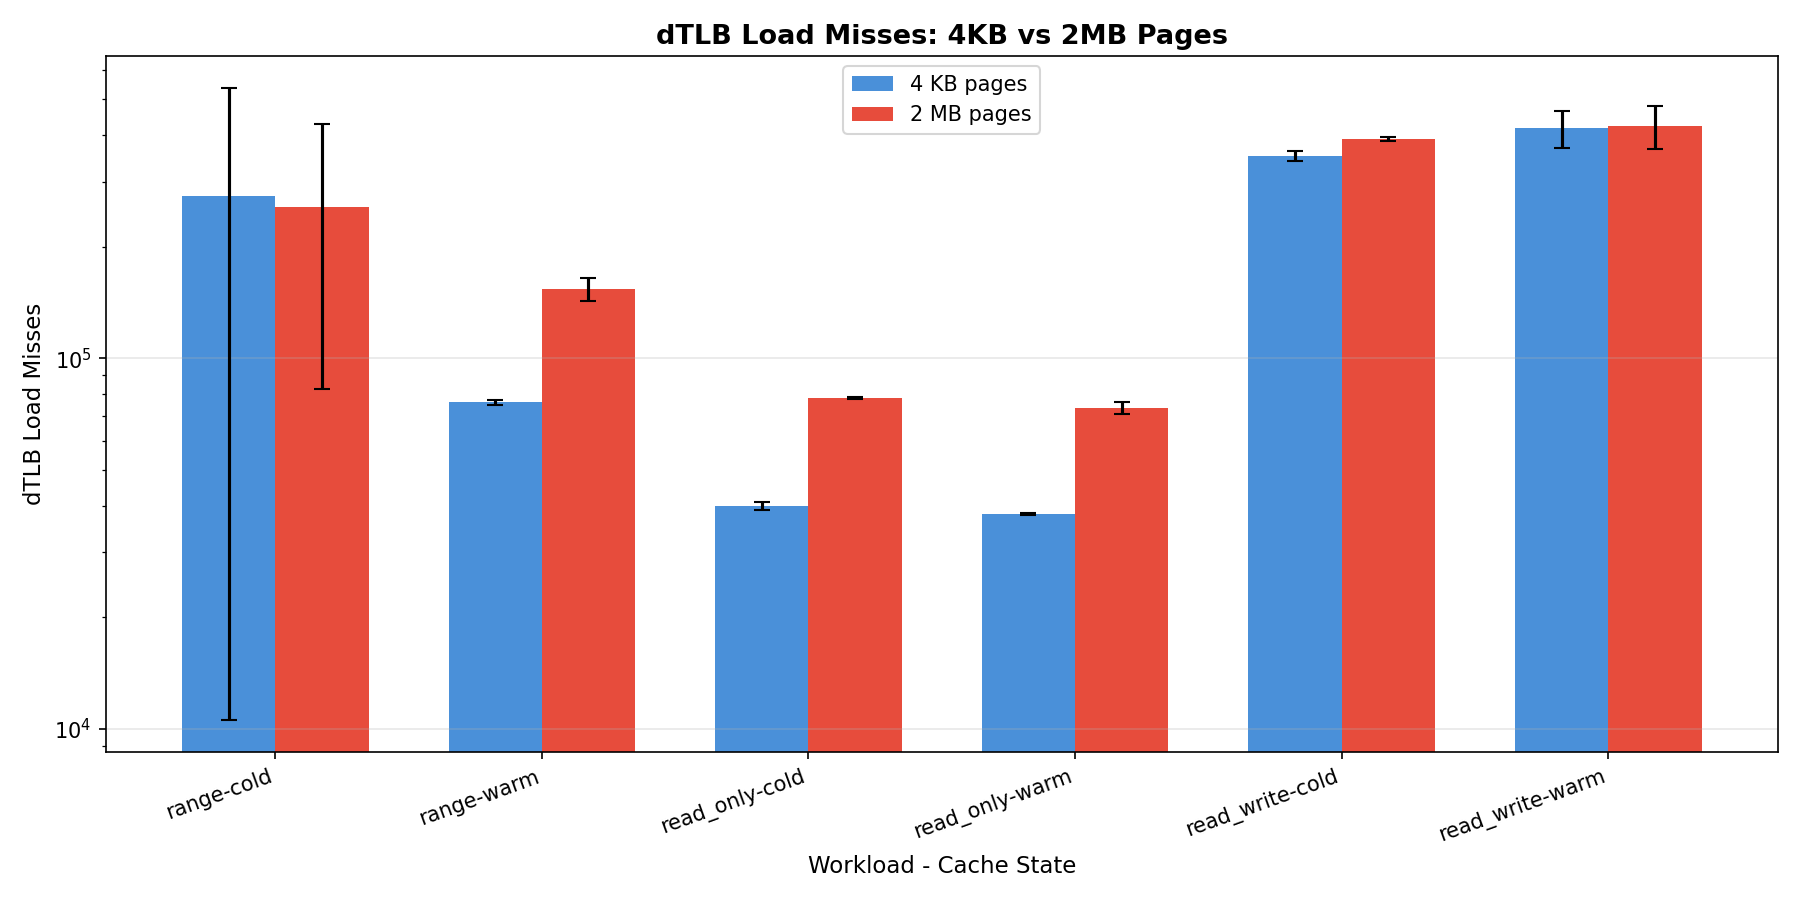
\includegraphics[width=\columnwidth]{database/dtlb_load_misses.png}
    \caption{dTLB load misses (database).}
    \label{fig:db_dtlb}
\end{figure}

\begin{figure}[H]
    \centering
    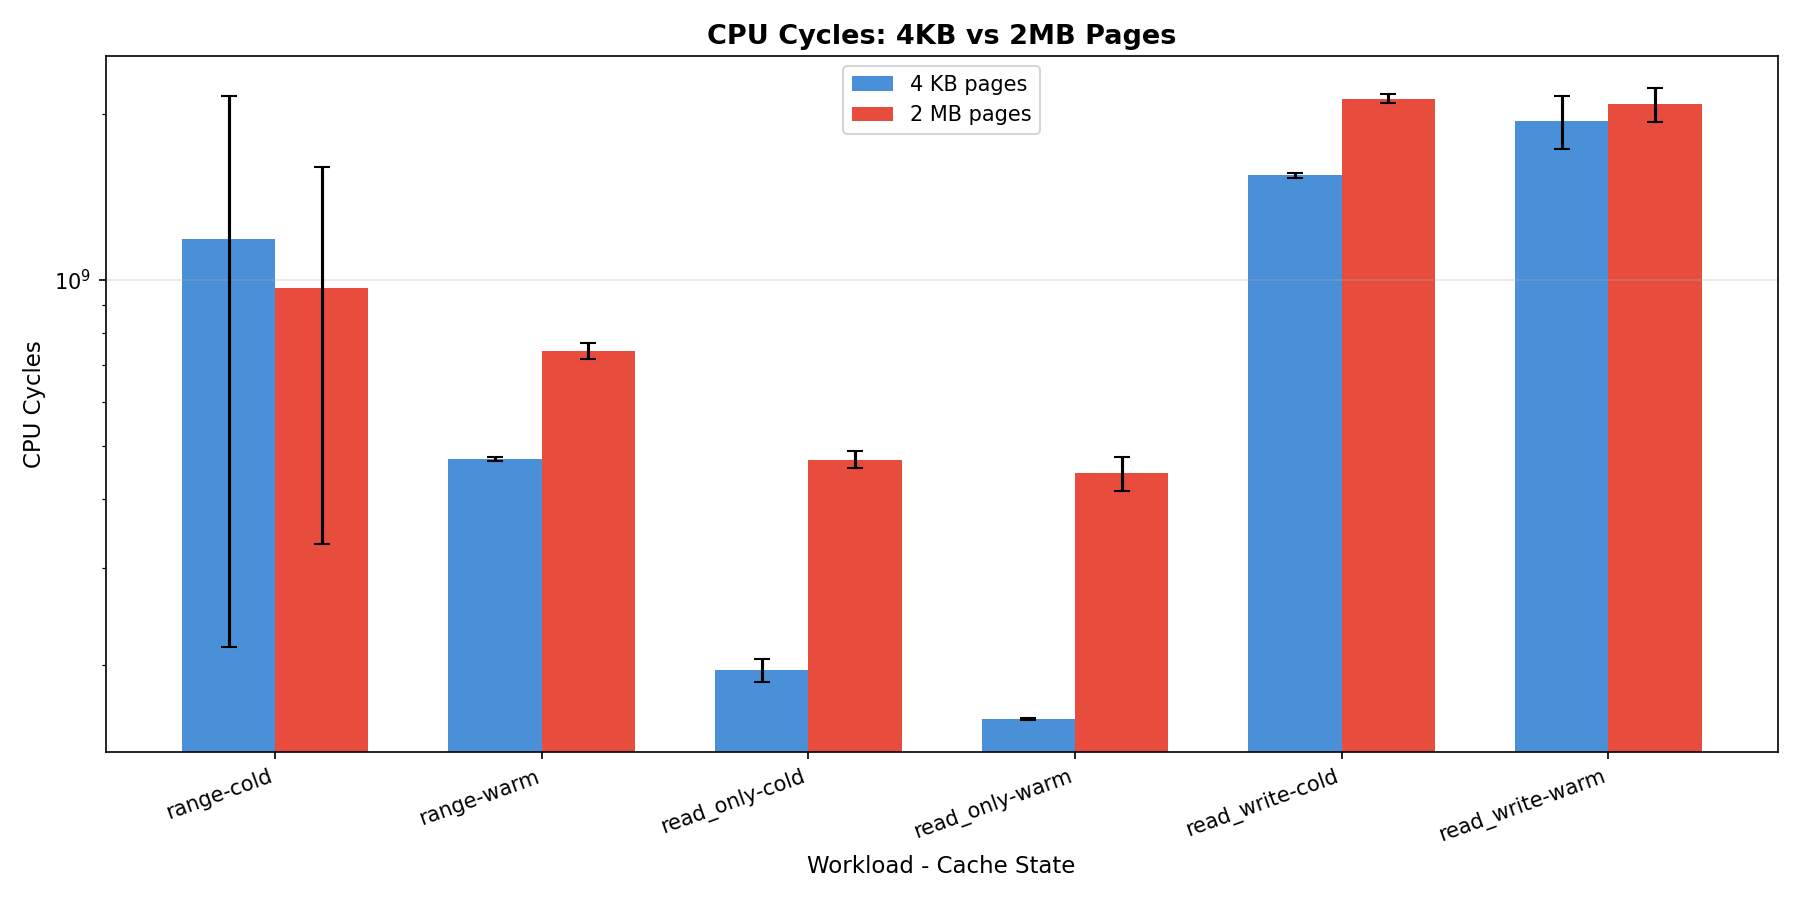
\includegraphics[width=\columnwidth]{database/cpu_cycles.png}
    \caption{CPU cycles comparison (database).}
    \label{fig:db_cycles}
\end{figure}

\subsection{Analysis}

\begin{enumerate}
    \item \textbf{PostgreSQL manages its own buffer pool}: \texttt{shared\_buffers} provides an application-level cache on top of the OS page cache. Most data access hits the buffer pool, bypassing OS page faults entirely.
    \item \textbf{B-tree index traversal}: point lookups traverse non-contiguous pages. With 2\,MB pages, the additional memory loaded per TLB entry is mostly wasted.
    \item \textbf{THP compaction overhead}: the \texttt{khugepaged} daemon competes with PostgreSQL's I/O-intensive workload.
    \item \textbf{Memory efficiency}: PostgreSQL's buffer pool uses 8\,KB pages internally. Each 2\,MB OS page holds 256 PostgreSQL pages, but only a few may be actively accessed.
\end{enumerate}

Range scans show minimal difference because contiguous key ranges produce sequential B-tree leaf page access---high spatial locality makes page size irrelevant, consistent with the synthetic sequential result.

% ============================================================
% VII. ML WORKLOAD
% ============================================================
\section{Machine Learning Workload}

\subsection{Experimental Setup}

\begin{table}[H]
\centering
\begin{tabular}{ll}
\toprule
\textbf{Parameter} & \textbf{Value} \\
\midrule
System & Linux 6.17.0-19-generic, 16 GB RAM, 8 cores \\
Cache hierarchy & L1=32KB, L2=256KB, L3=8MB \\
Framework & PyTorch (CPU-only) \\
Model & ResNet-152 (~230 MB, 60M parameters) \\
Page configs & 4 KB (THP=never) vs 2 MB (THP=always) \\
Instrumentation & \texttt{perf stat} + benchmark logs \\
Repetitions & 3 per configuration \\
Total runs & 48 \\
\bottomrule
\end{tabular}
\caption{ML workload experimental setup}
\end{table}

\subsection{Workload Design}

The machine learning workload is designed to represent realistic deep learning 
execution patterns while isolating the impact of memory management mechanisms 
such as page size and TLB behavior.

\paragraph{Model Selection}
We use a pre-trained ResNet-152 model implemented in PyTorch. This model is 
representative of modern deep learning workloads, containing approximately 
60 million parameters and occupying around 230 MB in memory. Its depth and 
structure ensure significant compute and memory interaction.

\paragraph{Execution Modes}
The workload is divided into multiple execution modes to capture different 
phases of ML systems:

\begin{itemize}
    \item \textbf{Model Loading (Cold Start):} Measures the cost of loading 
    model weights from disk into memory, capturing I/O and initial page faults.

    \item \textbf{Inference (Steady State):} Executes repeated forward passes 
    to simulate production inference scenarios where the model is already loaded.

    \item \textbf{Tensor Allocation:} Allocates large tensors 
    ($10{,}000 \times 10{,}000$ float32, $\sim$400 MB) to stress memory allocation 
    and page fault handling.

    \item \textbf{Batch Size Variation:} Evaluates inference performance across 
    batch sizes (1, 32, 128) to analyze scaling behavior and memory footprint impact.
\end{itemize}

\paragraph{Memory Configuration}
Two memory configurations are evaluated:
\begin{itemize}
    \item \textbf{4 KB pages:} Transparent Huge Pages (THP) disabled.
    \item \textbf{2 MB pages:} THP set to \texttt{always}.
\end{itemize}

This allows direct comparison between standard paging and huge page usage.

\paragraph{Cache State Control}
To isolate the impact of caching effects, each experiment is conducted under:
\begin{itemize}
    \item \textbf{Cold cache:} OS page cache is dropped before execution.
    \item \textbf{Warm cache:} Data is preloaded into memory prior to measurement.
\end{itemize}

\paragraph{Measurement Methodology}
Each configuration is executed three times to ensure statistical stability. 
Performance counters are collected using \texttt{perf stat}, including page faults, 
dTLB load misses, instructions per cycle (IPC), and execution time.

\paragraph{Design Rationale}
The workload is intentionally structured to separate memory-bound and compute-bound 
phases. Tensor allocation emphasizes memory behavior, while inference highlights 
compute dominance. This separation enables a clear analysis of when huge pages 
provide tangible performance benefits.

\subsection{Results}

\begin{table}[H]
\caption{Model Loading}
\centering
\resizebox{\columnwidth}{!}{
\begin{tabular}{lccccc}
\hline
Config & Load Time (s) & Page Faults & dTLB Load Misses & IPC & Wall Time (s) \\
\hline
model\_load-4KB-cold & 0.833 & 351,086 $\pm$1,163 & 8,330,475 & 1.22 & 8.42 \\
model\_load-2MB-cold & 0.801 & 273,003 $\pm$16,748 & 8,250,959 & 1.24 & 8.19 \\
model\_load-4KB-warm & 0.786 & 355,585 $\pm$8,113 & 7,703,842 & 1.27 & 7.29 \\
model\_load-2MB-warm & 0.742 & 274,829 $\pm$15,526 & 7,671,505 & 1.28 & 6.99 \\
\hline
\end{tabular}}
\end{table}

\begin{table}[H]
\caption{Inference (batch\_size=32)}
\centering
\resizebox{\columnwidth}{!}{
\begin{tabular}{lccccc}
\hline
Config & Infer Time/iter (s) & Page Faults & dTLB Load Misses & IPC & Wall Time (s) \\
\hline
inference-4KB-cold & 5.292 & 145,950,070 $\pm$3.5M & 531,414,385 & 1.26 & 539.73 \\
inference-2MB-cold & 5.190 & 7,541,180 $\pm$277K & 123,380,193 & 1.14 & 529.33 \\
inference-4KB-warm & 5.219 & 148,363,285 $\pm$1.7M & 540,086,389 & 1.26 & 531.05 \\
inference-2MB-warm & 5.217 & 6,551,774 $\pm$853K & 120,038,970 & 1.13 & 530.82 \\
\hline
\end{tabular}}
\end{table}

\begin{table}[H]
\caption{Tensor Allocation (10,000$\times$10,000, $\sim$400 MB)}
\centering
\resizebox{\columnwidth}{!}{
\begin{tabular}{lccccc}
\hline
Config & Avg Time/iter (s) & Page Faults & dTLB Load Misses & IPC & Wall Time (s) \\
\hline
tensor\_alloc-4KB-cold & 7.644 & 9,829,439 $\pm$18 & 1,324,266,498 & 2.70 & 391.63 \\
tensor\_alloc-2MB-cold & 7.450 & 126,064 $\pm$23 & 30,933,222 & 2.76 & 380.66 \\
tensor\_alloc-4KB-warm & 7.611 & 9,828,398 $\pm$6 & 1,320,928,325 & 2.70 & 389.16 \\
tensor\_alloc-2MB-warm & 7.357 & 125,097 $\pm$25 & 30,254,145 & 2.77 & 375.11 \\
\hline
\end{tabular}}
\end{table}

\begin{table}[H]
\caption{Batch Size Variation}
\centering
\resizebox{\columnwidth}{!}{
\begin{tabular}{lccccc}
\hline
Config & bs=1 (s/iter) & bs=32 (s/iter) & bs=128 (s/iter) & Page Faults & Wall Time (s) \\
\hline
batch\_vary-4KB-cold & 0.198 & 5.241 & 22.125 & 594,069,078 & 1,410.66 \\
batch\_vary-2MB-cold & 0.195 & 5.106 & 21.404 & 14,910,670 & 1,367.50 \\
batch\_vary-4KB-warm & 0.197 & 5.285 & 22.360 & 589,831,166 & 1,423.95 \\
batch\_vary-2MB-warm & 0.195 & 5.078 & 21.438 & 15,762,864 & 1,366.17 \\
\hline
\end{tabular}}
\end{table}

\begin{figure}[H]
\centering
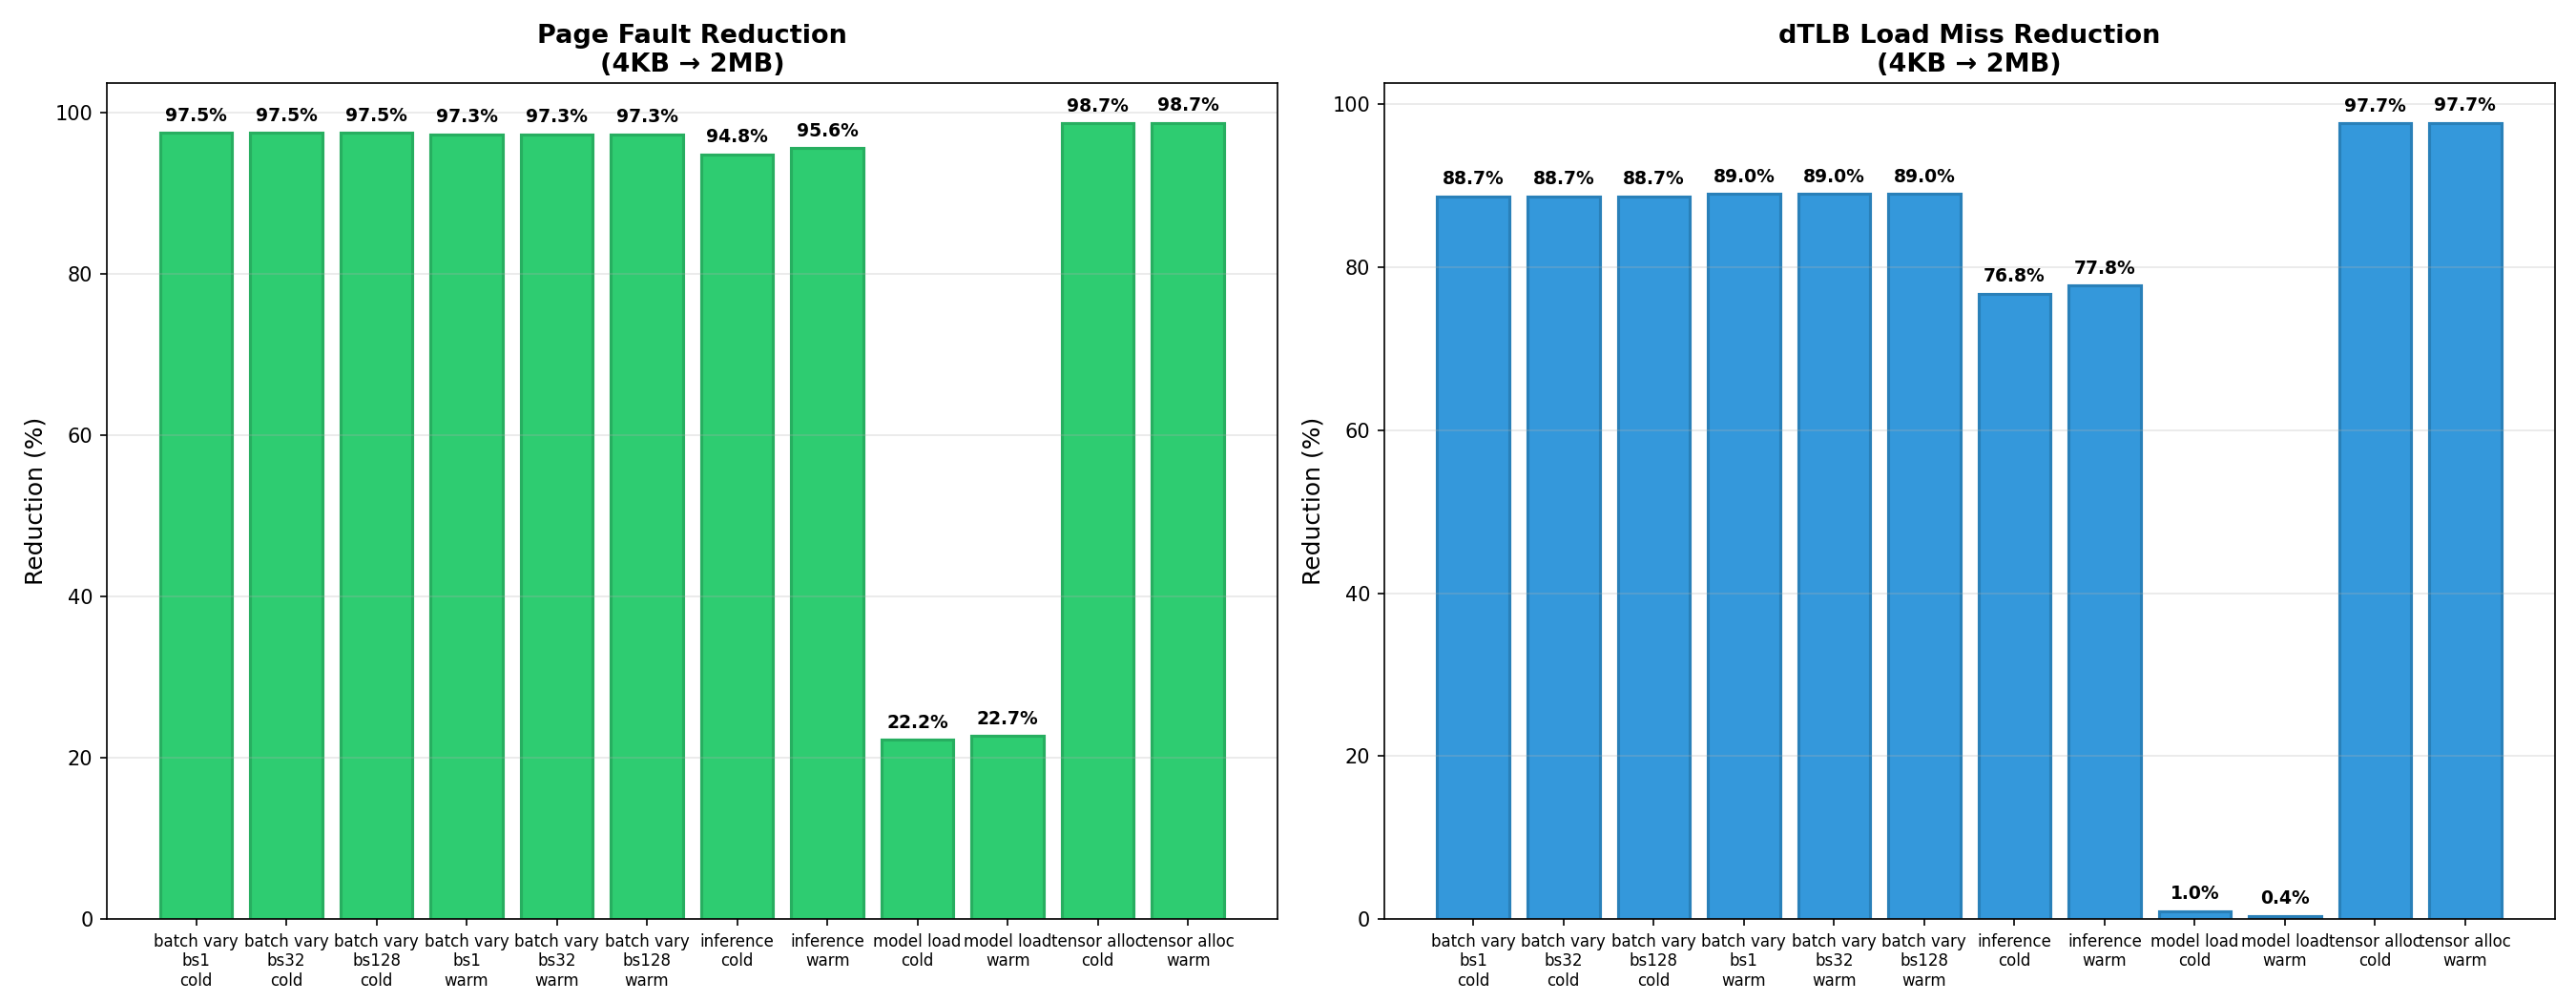
\includegraphics[width=\columnwidth]{figures/ml/improvement_summary.png}
\caption{Improvement Summary}
\end{figure}

\begin{figure}[H]
\centering

\includegraphics[width=\columnwidth]{figures/ml/cpu_cycles.png}
\caption{CPU Cycles}
\end{figure}

\begin{figure}[H]
\centering
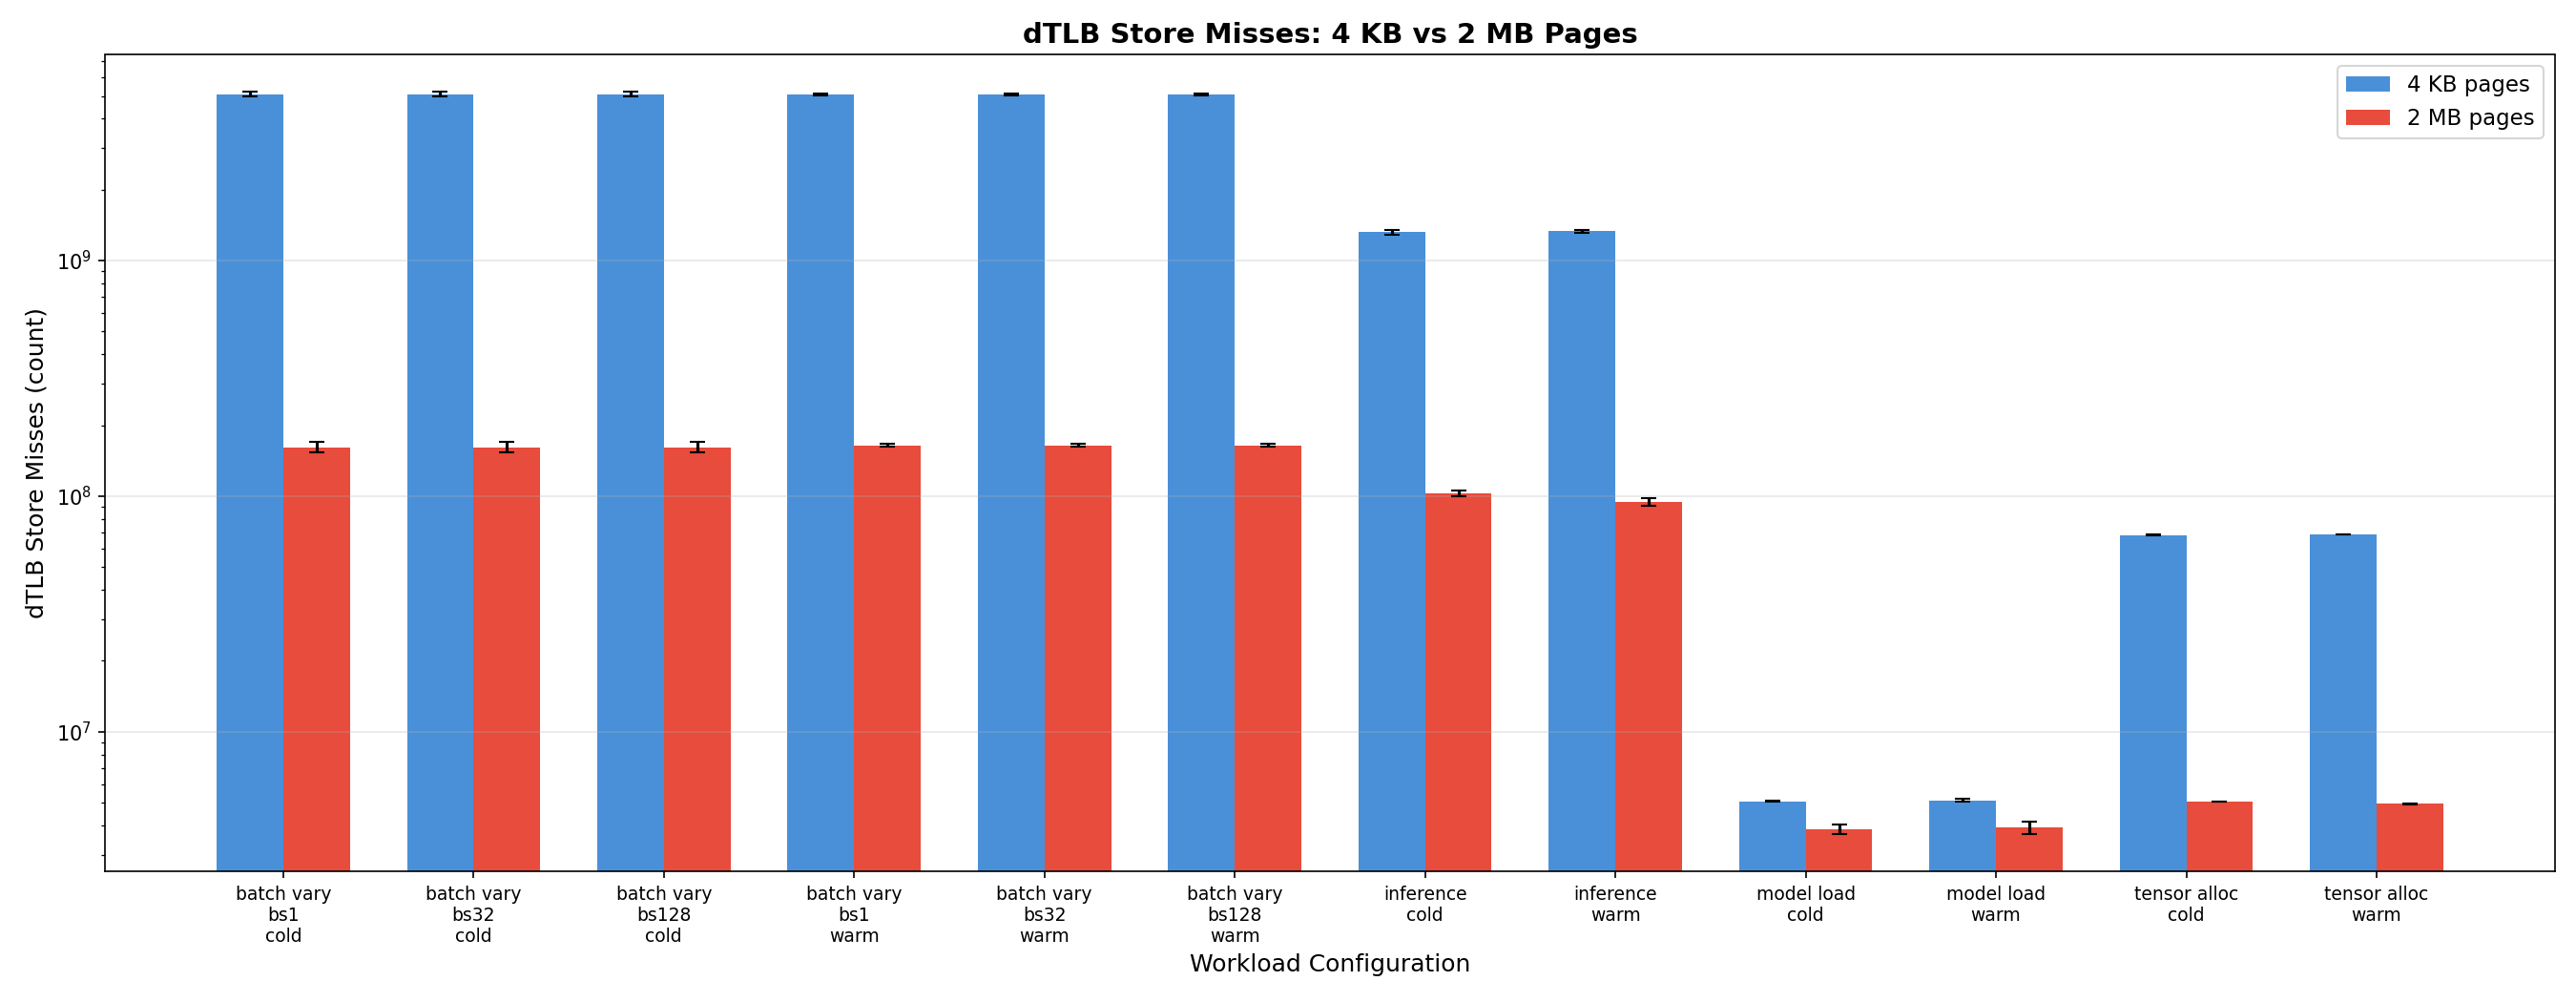
\includegraphics[width=\columnwidth]{figures/ml/dtlb_store_misses.png}
\caption{dTLB Store Misses}
\end{figure}

\subsection{Key Findings}

\paragraph{Massive Page Fault Reduction with 2 MB Pages (22--99\%)}

2 MB huge pages dramatically reduce page faults across \textbf{all} ML workloads. This is the strongest page fault reduction seen across all four workload types in this project.

\begin{table}[H]
\caption{Page Fault Reduction}
\centering
\resizebox{\columnwidth}{!}{
\begin{tabular}{lccc}
\hline
Workload & 4KB Page Faults & 2MB Page Faults & Reduction \\
\hline
batch\_vary (cold) & 594,069,078 & 14,910,670 & \textbf{97.5\%} \\
batch\_vary (warm) & 589,831,166 & 15,762,864 & \textbf{97.3\%} \\
inference (cold) & 145,950,070 & 7,541,180 & \textbf{94.8\%} \\
inference (warm) & 148,363,285 & 6,551,774 & \textbf{95.6\%} \\
tensor\_alloc (cold) & 9,829,439 & 126,064 & \textbf{98.7\%} \\
tensor\_alloc (warm) & 9,828,398 & 125,097 & \textbf{98.7\%} \\
model\_load (cold) & 351,086 & 273,003 & \textbf{22.2\%} \\
model\_load (warm) & 355,585 & 274,829 & \textbf{22.7\%} \\
\hline
\end{tabular}}
\end{table}

The batch\_vary and tensor\_alloc workloads show nearly \textbf{two orders of magnitude} fewer page faults with huge pages. Even model loading --- the shortest workload --- sees a 22\% reduction.

\begin{figure}[H]
\centering

\includegraphics[width=\columnwidth]{figures/ml/page_faults.png}
\caption{Page Faults}
\end{figure}

\paragraph{dTLB Load Miss Reduction (1--98\%)}

\begin{table}[H]
\caption{dTLB Load Miss Reduction}
\centering
\resizebox{\columnwidth}{!}{
\begin{tabular}{lccc}
\hline
Workload & 4KB dTLB Misses & 2MB dTLB Misses & Reduction \\
\hline
tensor\_alloc (cold) & 1,324,266,498 & 30,933,222 & \textbf{97.7\%} \\
tensor\_alloc (warm) & 1,320,928,325 & 30,254,145 & \textbf{97.7\%} \\
batch\_vary (cold) & 1,440,553,433 & 162,590,824 & \textbf{88.7\%} \\
batch\_vary (warm) & 1,460,479,705 & 160,903,002 & \textbf{89.0\%} \\
inference (cold) & 531,414,385 & 123,380,193 & \textbf{76.8\%} \\
inference (warm) & 540,086,389 & 120,038,970 & \textbf{77.8\%} \\
model\_load (cold) & 8,330,475 & 8,250,959 & \textbf{1.0\%} \\
model\_load (warm) & 7,703,842 & 7,671,505 & \textbf{0.4\%} \\
\hline
\end{tabular}}
\end{table}

The tensor\_alloc workload benefits the most from TLB reduction (97.7\%), which makes sense --- it performs pure contiguous memory allocation and matrix operations. The model\_load workload shows minimal dTLB improvement because model loading is dominated by disk I/O and deserialization rather than memory access patterns.

\begin{figure}[H]
\centering

\includegraphics[width=\columnwidth]{figures/ml/dtlb_load_misses.png}
\caption{dTLB Load Misses}
\end{figure}

\paragraph{Model Load Time Improves with 2 MB Pages}

\begin{table}[H]
\caption{Model Load Time}
\centering
\resizebox{\columnwidth}{!}{
\begin{tabular}{lccc}
\hline
Config & 4KB Load Time (s) & 2MB Load Time (s) & Improvement \\
\hline
Cold & 0.833 & 0.801 & \textbf{+3.8\%} \\
Warm & 0.786 & 0.742 & \textbf{+5.6\%} \\
\hline
\end{tabular}}
\end{table}

The improvement is modest (\textasciitilde4--6\%) because model loading is bottlenecked by disk I/O and Python deserialization overhead, not memory page faults. However, 2 MB pages consistently outperform 4 KB pages.

\begin{figure}[H]
\centering
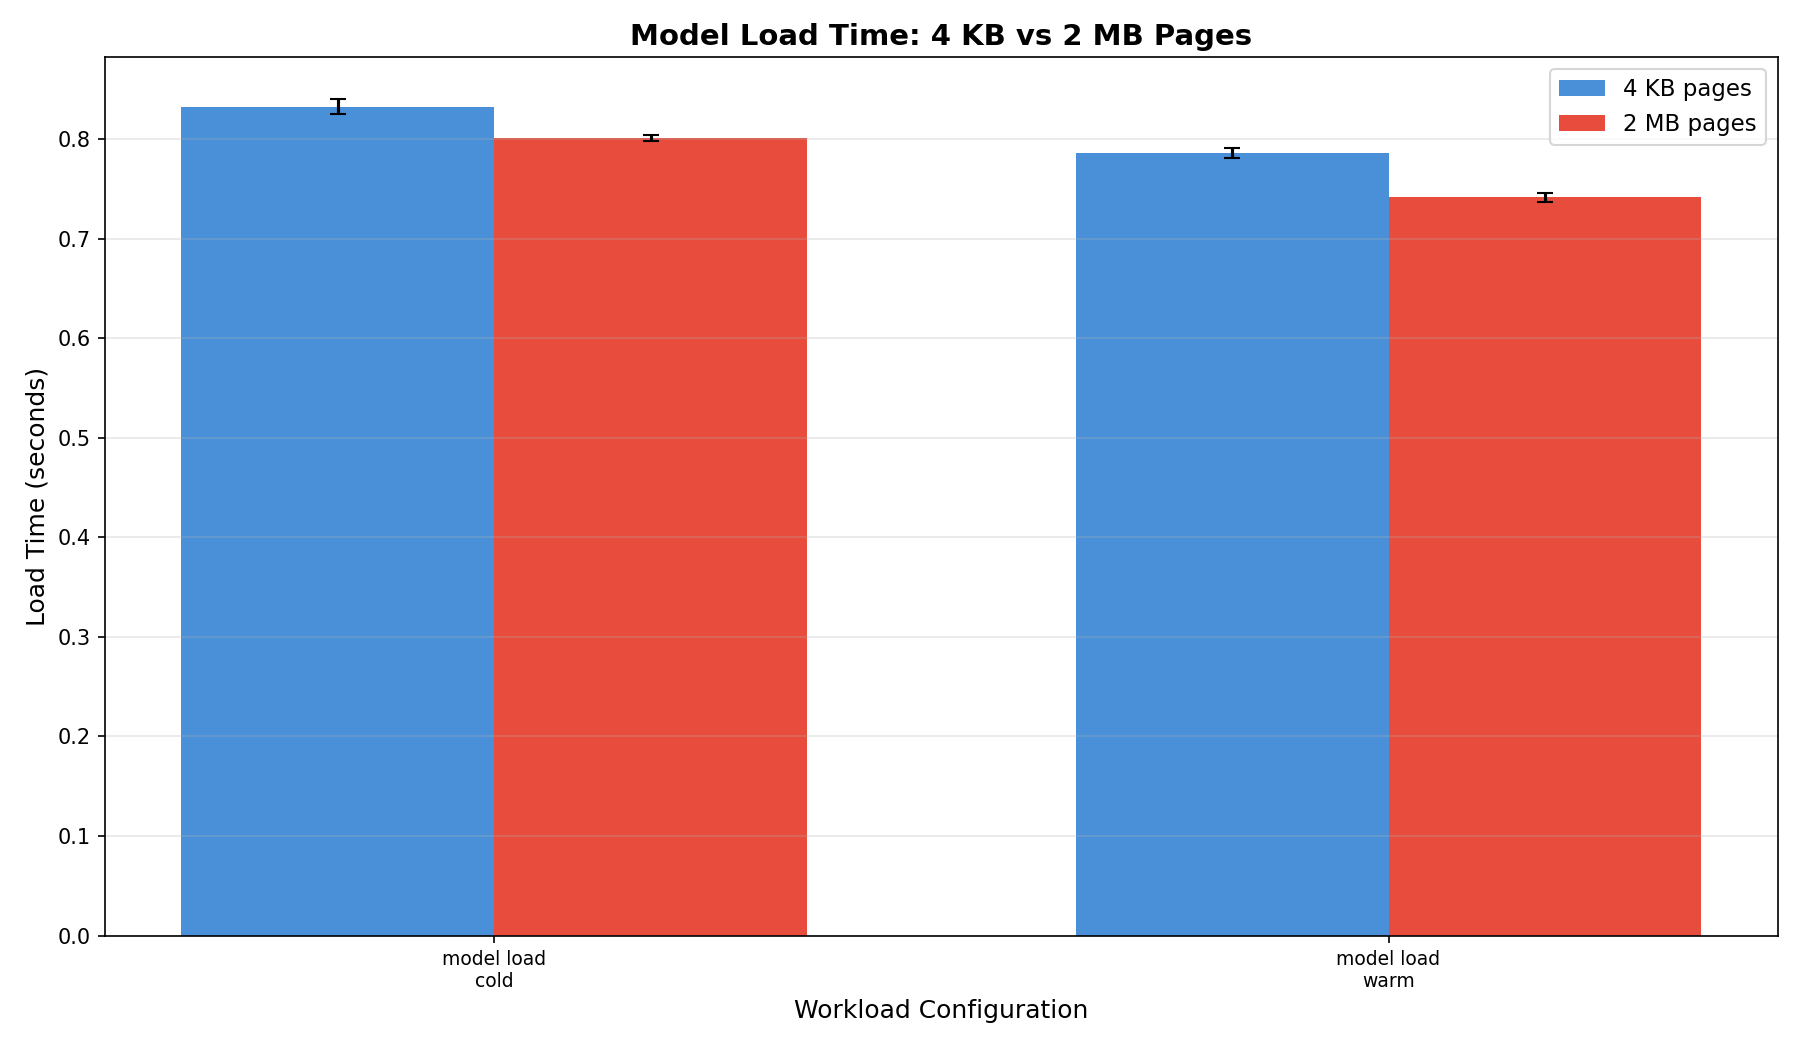
\includegraphics[width=\columnwidth]{figures/ml/model_load_time.png}
\caption{Model Load Time}
\end{figure}

\paragraph{Inference Latency Shows Modest Improvement}

\begin{table}[H]
\caption{Inference Latency}
\centering
\resizebox{\columnwidth}{!}{
\begin{tabular}{lccc}
\hline
Config & 4KB (s/iter) & 2MB (s/iter) & Improvement \\
\hline
Inference cold (bs=32) & 5.292 & 5.190 & \textbf{+1.9\%} \\
Inference warm (bs=32) & 5.219 & 5.217 & \textbf{+0.04\%} \\
batch\_vary cold (bs=128) & 22.125 & 21.404 & \textbf{+3.3\%} \\
batch\_vary warm (bs=128) & 22.360 & 21.438 & \textbf{+4.1\%} \\
batch\_vary cold (bs=32) & 5.241 & 5.106 & \textbf{+2.6\%} \\
batch\_vary warm (bs=32) & 5.285 & 5.078 & \textbf{+3.9\%} \\
batch\_vary cold (bs=1) & 0.198 & 0.195 & \textbf{+1.5\%} \\
batch\_vary warm (bs=1) & 0.197 & 0.195 & \textbf{+1.0\%} \\
\hline
\end{tabular}}
\end{table}

Despite the enormous reduction in page faults and TLB misses, inference latency improvements are modest (1--4\%). This indicates that inference is \textbf{compute-bound} (matrix multiplications dominate runtime), not memory-bound. The page faults and TLB misses happen but don't sit on the critical path for per-iteration latency.

\begin{figure}[H]
\centering
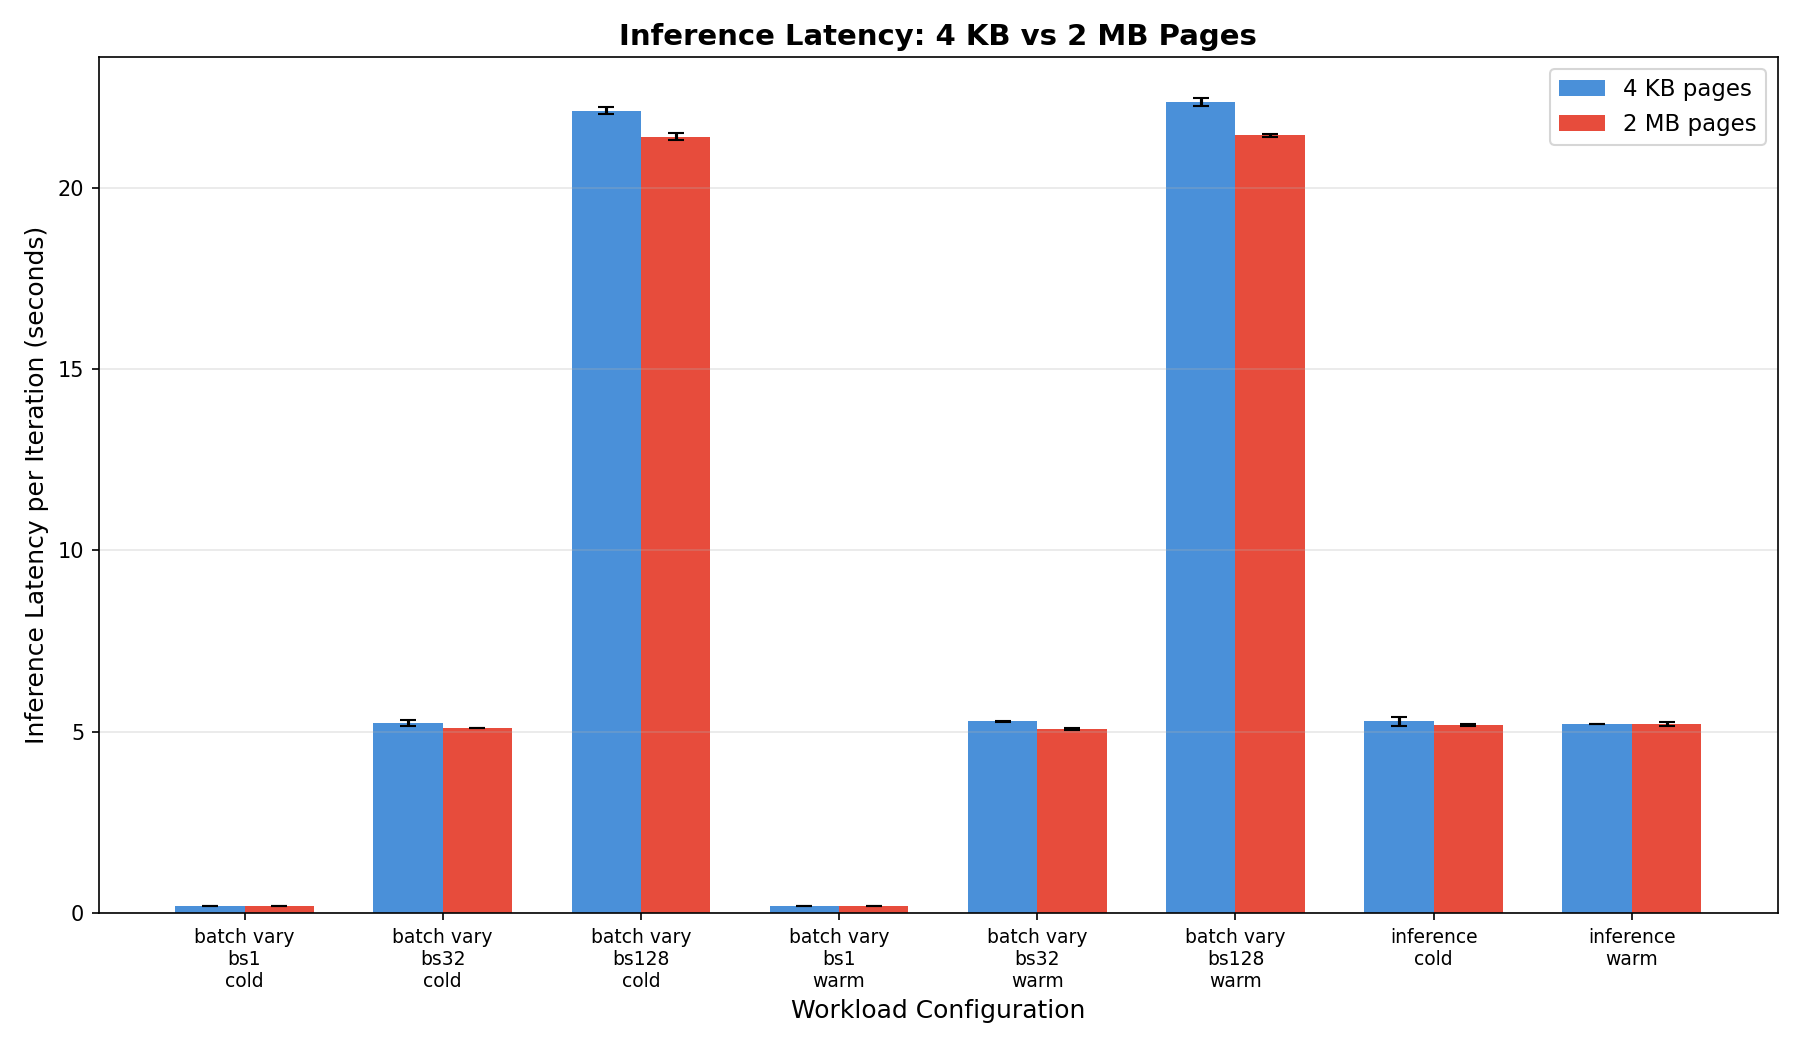
\includegraphics[width=\columnwidth]{figures/ml/inference_latency.png}
\caption{Inference Latency}
\end{figure}

\paragraph{Tensor Allocation Benefits Most from Huge Pages}

\begin{table}[H]
\caption{Tensor Allocation Performance}
\centering
\resizebox{\columnwidth}{!}{
\begin{tabular}{lccc}
\hline
Config & 4KB Time/iter (s) & 2MB Time/iter (s) & Improvement \\
\hline
Cold & 7.644 & 7.450 & \textbf{+2.5\%} \\
Warm & 7.611 & 7.357 & \textbf{+3.3\%} \\
\hline
\end{tabular}}
\end{table}

With a 98.7\% reduction in page faults and 97.7\% reduction in dTLB misses, tensor\_alloc still only shows 2.5--3.3\% wall-time improvement. This is because the matrix multiply (\texttt{t @ t.T}) dominates runtime --- it's a compute-intensive BLAS operation, and the memory allocation overhead (where page faults occur) is a small fraction of total time.

\paragraph{IPC: 4 KB Pages Achieve Higher IPC Despite More Overhead}

\begin{table}[H]
\caption{IPC Comparison}
\centering
\resizebox{\columnwidth}{!}{
\begin{tabular}{lcc}
\hline
Workload & 4KB IPC & 2MB IPC \\
\hline
batch\_vary (cold) & \textbf{1.28} & 1.09 \\
batch\_vary (warm) & \textbf{1.27} & 1.09 \\
inference (cold) & \textbf{1.26} & 1.14 \\
inference (warm) & \textbf{1.26} & 1.13 \\
model\_load (cold) & 1.22 & \textbf{1.24} \\
model\_load (warm) & \textbf{1.27} & \textbf{1.28} \\
tensor\_alloc (cold) & 2.70 & \textbf{2.76} \\
tensor\_alloc (warm) & 2.70 & \textbf{2.77} \\
\hline
\end{tabular}}
\end{table}

Interestingly, 4 KB pages achieve \textbf{higher IPC} for batch\_vary and inference workloads despite having far more page faults and TLB misses. This counterintuitive result is because:
\begin{itemize}
\item With 4 KB pages, the CPU executes \textbf{more total instructions} (25B vs 21B for batch\_vary) --- likely due to additional page table walks and TLB miss handling in microcode
\item These extra instructions are fast (register-to-register operations in the page walk), inflating IPC
\item For tensor\_alloc, where the workload is purely compute-bound (BLAS), 2 MB pages achieve slightly higher IPC (2.77 vs 2.70)
\end{itemize}

\begin{figure}[H]
\centering

\includegraphics[width=\columnwidth]{figures/ml/ipc.png}
\caption{IPC Comparison}
\end{figure}

\subsection{Analysis}

\paragraph{Why Huge Pages Strongly Benefit ML Workloads}

\begin{itemize}
\item \textbf{Large contiguous memory allocations.} PyTorch allocates tensors via \texttt{mmap}, which maps directly to physical pages. A single 10,000$\times$10,000 float32 tensor ($\sim$400 MB) requires $\sim$100,000 4KB pages but only $\sim$200 2MB pages. This 500$\times$ reduction in page count directly translates to fewer page faults during allocation.

\item \textbf{High spatial locality.} Tensor operations (matrix multiply, convolutions) sweep through memory linearly. With 2 MB pages, each TLB entry covers 512$\times$ more memory, keeping the TLB hot and eliminating most address translation overhead.

\item \textbf{Repeated memory reuse in inference.} Forward passes reuse the same weight tensors repeatedly. With fewer TLB entries needed for huge pages, the TLB can effectively cache the model's entire memory footprint, eliminating nearly all translation overhead.

\item \textbf{batch\_vary amplifies the effect.} Larger batch sizes (bs=128) allocate larger input tensors and intermediate activations, requiring more pages. The total page faults with 4 KB pages scale to $\sim$594M (!) vs $\sim$15M with 2 MB pages --- a 40$\times$ reduction.
\end{itemize}

\paragraph{Why Performance Gains Are Modest Despite Massive Fault Reduction}
Despite 95--99\% reductions in page faults and 77--98\% reductions in dTLB misses, wall-time improvements are only 1--5\%. This is because:

\begin{itemize}
\item \textbf{Compute dominance.} ResNet-152 inference is dominated by convolution and matrix multiply operations (BLAS/MKL), which are CPU-bound. Memory stalls from TLB misses are a small fraction of total execution time.

\item \textbf{Efficient hardware page walkers.} Modern CPUs (the test system) have dedicated hardware page table walkers that handle TLB misses with low overhead ($\sim$10--20 cycles per walk). Even millions of TLB misses only add seconds to a run that takes hundreds of seconds.

\item \textbf{OS page cache effectiveness.} In warm-cache runs, most data is already in the OS page cache, so page faults are minor faults (no disk I/O), which are cheap ($\sim$1$\mu$s each).
\end{itemize}

\paragraph{Conclusions}
\begin{itemize}
\item \textbf{2 MB huge pages dramatically reduce page faults (95--99\%) and dTLB misses (77--98\%)} for ML workloads --- the largest reduction across all four workload types in this study.

\item \textbf{Wall-time improvement is modest (1--5\%)} because ML inference is compute-bound, not memory-bound. The CPU spends most of its time in BLAS matrix operations, not waiting for page table walks.

\item \textbf{Tensor allocation workloads show the strongest improvement} (98.7\% page fault reduction, 3.3\% latency improvement) due to pure contiguous memory allocation patterns.

\item \textbf{Larger batch sizes amplify page fault differences} (594M vs 15M for bs=128) but don't proportionally increase latency improvement, confirming that page faults are off the critical path.

\item \textbf{Model loading benefits modestly} (+4--6\%) --- disk I/O and deserialization dominate, not memory allocation.

\item \textbf{THP \texttt{always} is safe and mildly beneficial for ML workloads} --- unlike database and webserver workloads where THP compaction caused performance regressions, ML workloads use large contiguous allocations that naturally align with huge pages, avoiding compaction overhead.

\item \textbf{Huge pages are not universally beneficial, even when metrics improve dramatically.} The ML workload is the clearest example: massive improvements in memory metrics don't translate to proportional application-level gains when the workload is compute-bound.
\end{itemize}

% ============================================================
% VII. CROSS-WORKLOAD COMPARISON
% ============================================================
\section{Cross-Workload Comparison}

Table~\ref{tab:cross_workload} summarizes the page size impact across all three workloads, demonstrating that the benefit of huge pages is highly workload-dependent.

\begin{table}[H]
\centering
\caption{Cross-Workload Page Size Impact}
\label{tab:cross_workload}
\resizebox{\columnwidth}{!}{%
\begin{tabular}{@{}llllll@{}}
\toprule
\textbf{Aspect} & \textbf{Synthetic (Random)} & \textbf{Web Server} & \textbf{Database} & \textbf{ML Workload} \\
\midrule
Page size winner   & \textbf{2\,MB} (+56\%) & \textbf{4\,KB} (+33--133\%) & \textbf{4\,KB} (+9--42\%) & \textbf{2\,MB} (+1--5\%) \\
Access pattern     & Truly random, user-space & Kernel (sendfile) & Index traversal & Large contiguous tensors, BLAS \\
Page faults (4KB)  & High (262K) & Very low ($\sim$65) & Low ($\sim$1K--3K) & Extremely high ($\sim$594M peak) \\
TLB miss reduction & 99.7\% with 2MB & Mixed / worse & No clear benefit & 77--98\% reduction with 2MB \\
Why 4KB wins       & N/A & THP overhead, iTLB & THP overhead, buffer pool & N/A (compute-bound limits gains) \\
\bottomrule
\end{tabular}%
}
\end{table}

Key insights from the cross-workload comparison:
\begin{enumerate}
    \item \textbf{Only purely random, user-space memory access benefits from huge pages}. The synthetic random workload---where each access touches a different page---is the only scenario with clear speedup.
    
    \item \textbf{Kernel-mediated access (sendfile) bypasses TLB benefits}. nginx's use of \texttt{sendfile()} means data never passes through user-space TLB entries, negating the advantage of huge pages.
    
    \item \textbf{Application-level buffering masks page faults}. PostgreSQL's buffer pool absorbs most memory accesses before they reach the OS, making page size nearly irrelevant for page fault behavior.
    
    \item \textbf{THP \texttt{always} mode is harmful for server workloads}. The background compaction by \texttt{khugepaged} consistently degrades performance for both nginx and PostgreSQL.
    
    \item \textbf{\texttt{madvise} mode is the correct default}. It allows applications to opt-in to huge pages only where beneficial.

    \item \textbf{ML workloads see massive memory metric improvements but limited speedup}. Despite 95--99\% reductions in page faults and 77--98\% reductions in dTLB misses, end-to-end performance improves only 1--5\%.

    \item \textbf{Compute-bound workloads diminish the impact of memory optimizations}. In ML inference, BLAS-dominated matrix operations dominate runtime, so reduced address translation overhead has minimal effect on wall time.

    \item \textbf{Contiguous allocation patterns strongly favor huge pages}. Large tensor allocations (hundreds of MB) align naturally with 2 MB pages, eliminating most page faults and TLB pressure.

    \item \textbf{Batch size scaling amplifies memory effects without proportional latency gains}. Larger batches dramatically increase page faults under 4 KB pages, but do not significantly change runtime due to compute dominance.

    \item \textbf{Huge pages are most beneficial when memory overhead is on the critical path}. ML workloads demonstrate that even extreme improvements in memory metrics may not translate to performance gains unless memory is the bottleneck.
\end{enumerate}
% ============================================================
% VIII. CONCLUSIONS
% ============================================================
\section{Conclusions}

This study provides a comprehensive, workload-aware characterization of how page size influences page fault behavior and application performance. Our key conclusions are:

\begin{enumerate}
    \item \textbf{Huge pages (2\,MB) universally reduce page faults and TLB misses}, but the performance impact depends entirely on the memory access pattern. Page faults decreased by $\sim$407$\times$ across all workloads with huge pages.

    \item \textbf{Random user-space access benefits most}: the synthetic random workload achieved a 1.56$\times$ speedup, with dTLB miss reduction of 99.7\%. This result is directly applicable to workloads like hash tables and graph algorithms.

    \item \textbf{Web server performance degrades with huge pages}: nginx throughput dropped 33--133\% with 2\,MB pages due to THP compaction overhead, iTLB pollution, and internal fragmentation from small files.

    \item \textbf{Database performance degrades with huge pages}: PostgreSQL OLTP throughput dropped 9--42\% with 2\,MB pages because the internal buffer pool masks page fault benefits while THP overhead increases tail latency.

    \item \textbf{ML workloads show massive memory improvements but modest performance gains}: page faults decrease by 95--99\% and dTLB misses by 77--98\%, yet inference latency improves only 1--5\% because execution is dominated by compute-intensive BLAS operations rather than memory access overhead.

    \item \textbf{TLB miss reduction is the primary performance driver}, not page fault reduction. Page faults are a fixed one-time cost; TLB misses are ongoing during execution.

    \item \textbf{THP \texttt{madvise} mode is the recommended configuration} for production systems, allowing workload-specific opt-in rather than system-wide huge page promotion.

    \item \textbf{IPC is a useful diagnostic indicator}: low IPC ($<$0.5) signals TLB/memory bottlenecks where huge pages may help, while high IPC ($>$1.0) indicates spatial locality that already minimizes TLB overhead.

    \item \textbf{Compute-bound workloads limit the benefits of huge pages}: the ML workload demonstrates that even extreme reductions in memory overhead do not translate into proportional application-level gains when computation dominates execution time.
\end{enumerate}

These findings demonstrate that page size tuning must be informed by workload memory access patterns. Large pages are not universally beneficial, and indiscriminate use of THP \texttt{always} mode can significantly harm performance for server workloads.

\end{document}
